%%%%%%%%%%%%%%%%%%%%%%%%%%%%%%%%%%%%%%%%%%%%%%%%%%%%%%%%%%%%%%%%%%%%%%%%%%%%%%%%%%
\begin{frame}[fragile]\frametitle{}
\begin{center}
{\Large Statistical Testing}
\end{center}
\end{frame}

%%%%%%%%%%%%%%%%%%%%%%%%%%%%%%%%%%%%%%%%%%%%%%%%%%%
\begin{frame}[fragile]\frametitle{Tests}
\begin{center}

\includegraphics[width=\linewidth,keepaspectratio]{ttest}
\end{center}
\end{frame}


%%%%%%%%%%%%%%%%%%%%%%%%%%%%%%%%%%%%%%%%%%%%%%%%%%%%%%%%%%%
\begin{frame}[fragile]\frametitle{Hypothesis}
\begin{itemize}
\item Formulate effect/relation which needs to be tested
\item Null Hypothesis ($H_0$): Assume Guess/relation does not exist.
\item Alternate Hypothesis ($H_1$): Assume Guess/relation does exist. 
\item Eg. you are trying to state that your method has positive effect and there is some change.
\end{itemize}
\end{frame}

%%%%%%%%%%%%%%%%%%%%%%%%%%%%%%%%%%%%%%%%%%%%%%%%%%%%%%%%%%%
\begin{frame}[fragile]\frametitle{Hypothesis}
\begin{itemize}
\item Objective: Prove Null Hypothesis wrong.
\item Get enough evidence to disprove the Null Hypothesis.
\item {\bf Your never prove that $H_1$ is true, you can only reject $H_0$}
\end{itemize}
\end{frame}

%%%%%%%%%%%%%%%%%%%%%%%%%%%%%%%%%%%%%%%%%%%%%%%%%%%%%%%%%%%
\begin{frame}[fragile]\frametitle{Hypothesis}
Example:
\begin{itemize}
\item There is one distribution for $H_0$. 
\item There is another distribution for $H_1$
\item Your model will give some output distribution which one needs to check if its in $H_0$s acceptance region or rejection region, and how much?
\end{itemize}
\begin{center}
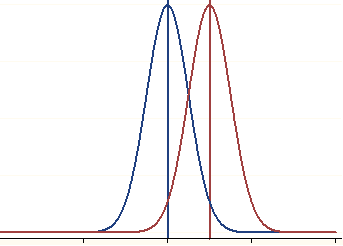
\includegraphics[width=0.5\linewidth,keepaspectratio]{distdiff}
\end{center}
\end{frame}


%%%%%%%%%%%%%%%%%%%%%%%%%%%%%%%%%%%%%%%%%%%%%%%%%%%%%%%%%%%
\begin{frame}[fragile]\frametitle{Errors}
\begin{itemize}
\item Whenever you reject a hypothesis, there is a chance that you make some errors there.
\item They care classified into Type I and Type II errors
\end{itemize}
\end{frame}

%%%%%%%%%%%%%%%%%%%%%%%%%%%%%%%%%%%%%%%%%%%%%%%%%%%%%%%%%%%
\begin{frame}[fragile]\frametitle{Errors}
\begin{itemize}
\item Type I: Incorrectly reject $H_0$. 
\item `Reject $H_0$', meaning $H_1$ can be accepted, which in turn talks about Test being positive.
\item But then `incorrectly' means Falsely , so the whole thing is False Positive.
\item Test is positive but it could actually be wrong. False Positives.
\item Probability of making Type I errors is $\alpha$
\end{itemize}
\end{frame}

%%%%%%%%%%%%%%%%%%%%%%%%%%%%%%%%%%%%%%%%%%%%%%%%%%%%%%%%%%%
\begin{frame}[fragile]\frametitle{Errors}
\begin{itemize}
\item Type II: Fail to reject $H_0$ when you should have done it. 
\item `reject $H_0$' meaning $H_1$ can be accepted, which in turn talks about Test being Positive.
\item `Fails to' do that means the Test came out negative. 
\item This should have been done, but did not happen, so `False'. So the whole thing is False Negative.
\item Test is negative but but it could actually be wrong, ie the disease is there. False Negative.
\item Probability of making Type II errors is $\beta$
\end{itemize}
\end{frame}


%%%%%%%%%%%%%%%%%%%%%%%%%%%%%%%%%%%%%%%%%%%%%%%%%%%%%%%%%%%%
%\begin{frame}[fragile]\frametitle{Some Required Definitions}
%\begin{itemize}
%\item Power: Probability of finding a difference between groups if one truly exists = $1 - \beta$. 
%\item Good to have High Power. 
%\item Having beta less that 20\%.
%\item Power increases as sample size increases, as you have more data to make conclusions.
%\item Power increases as difference between groups becomes more significant. Easy to differentiate.
%\item Power increases as precision increases (ie decrease in std deviation)
%\end{itemize}
%\end{frame}


%%%%%%%%%%%%%%%%%%%%%%%%%%%%%%%%%%%%%%%%%%%%%%%%%%%%%%%%%%%
\begin{frame}[fragile]\frametitle{Some Required Definitions}
\begin{itemize}
\item Normality: Most of the test assume that, the data or test statistics 
or some function in testing procedure under consideration follows 
Normal distribution. 
 
\item Decision  criteria: z critical values:  boundaries for rejection or non rejection region
\end{itemize}
\end{frame}

%%%%%%%%%%%%%%%%%%%%%%%%%%%%%%%%%%%%%%%%%%%%%%%%%%%%%%%%%%%
\begin{frame}
\begin{center}
{\Large P-Value}
\end{center}
\end{frame}



%%%%%%%%%%%%%%%%%%%%%%%%%%%%%%%%%%%%%%%%%%%%%%%%%%%%%%%%%%%%%%%%%%%%%%%%
\begin{frame}[fragile]\frametitle{P-Value}


	\begin{itemize}

	\item Do not confuse this p with probability. They are related but not the same.
	\item Experiment: What is the probability of getting 2 heads in a row? Whats the p-value of getting 2 heads in a row?
	\item Probability of getting 1 heads and 1 tails is $0.25 + 0.25 = 0.5$. Here order did not matter, ie HT and TH is same.
	
	\end{itemize}


      \begin{center}
      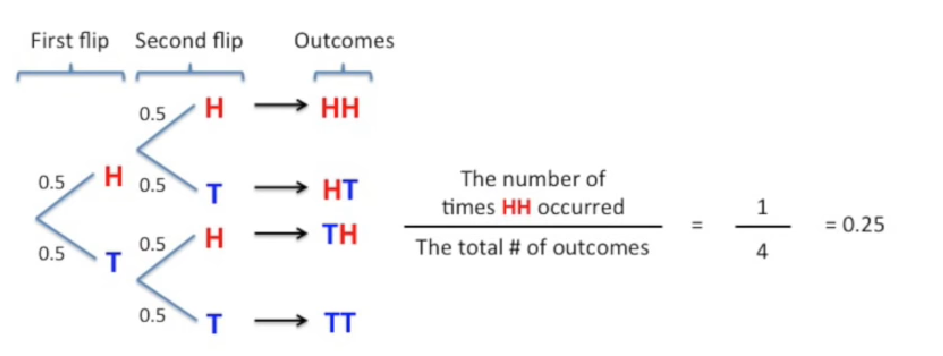
\includegraphics[width=\linewidth,keepaspectratio]{statq39}
	  	\end{center}

  
 
\tiny{(Ref: StatQuest: P Values, clearly explained - Josh Starmer )}
\end{frame}

%%%%%%%%%%%%%%%%%%%%%%%%%%%%%%%%%%%%%%%%%%%%%%%%%%%%%%%%%%%%%%%%%%%%%%%%
\begin{frame}[fragile]\frametitle{P-Value}

\begin{itemize}

	\item P-Value of getting HH?
	\item P-value is the probability that random chance generated data (which is 0.25) is equal (ie of TT, which has same probability, ie 0.25) or rarer (there are none here)
	\item So P-value for HH is 0.5
	
	\end{itemize}

      \begin{center}
      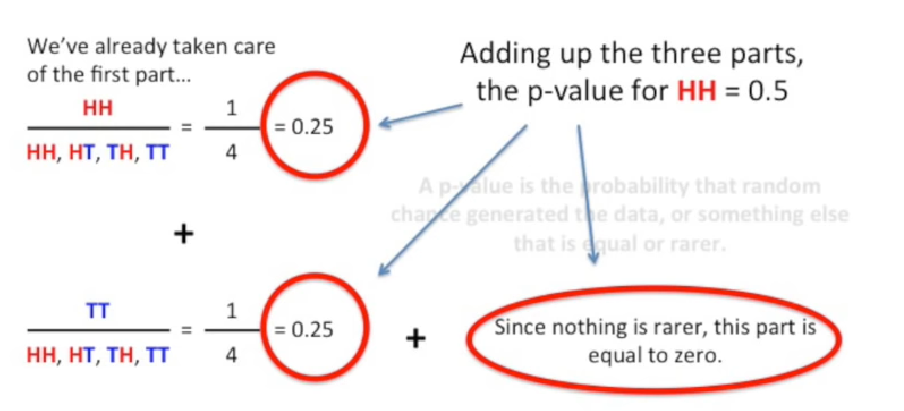
\includegraphics[width=\linewidth,keepaspectratio]{statq40}
	  	\end{center}

  
  
 
\tiny{(Ref: StatQuest: P Values, clearly explained - Josh Starmer )}
\end{frame}

%%%%%%%%%%%%%%%%%%%%%%%%%%%%%%%%%%%%%%%%%%%%%%%%%%%%%%%%%%%
\begin{frame}[fragile]\frametitle{Level of Significance: p-value}
\begin{itemize}
\item Level of Significance: Probability of rejecting null  
hypothesis when it is true. Represented by Greek letter `alpha'. 
\item if $p < \alpha$ : there is statistically significant difference between groups
\item if $p > \alpha$ : there is NOT MUCH statistically significant difference between groups
\item $\alpha$ is generally 0.05
\item So, only incorrectly rejecting $H_0$ is ok upto 5\%. 
\item Type I error only upto 5\%
\end{itemize}
\end{frame}

%%%%%%%%%%%%%%%%%%%%%%%%%%%%%%%%%%%%%%%%%%%%%%%%%%%%%%%%%%%
\begin{frame}[fragile]\frametitle{Level of Significance: p-value: Example}
 Why p-value is the deciding factor for accepting or rejecting a hypothesis we
develop before any experiment?
\begin{itemize}
\item You have launched a product (e.g. a phone) in the market. 
\item And you get customer feedback that the phone has over heating problem. 
\item As the phone is already launched in the market you can't recall all of them to test if the majority of the phones have overheating problem due to some manufacturing problem.
\end{itemize}

(Ref: https://www.datasciencecentral.com/profiles/blogs/significance-of-p-value)
\end{frame}


%%%%%%%%%%%%%%%%%%%%%%%%%%%%%%%%%%%%%%%%%%%%%%%%%%%%%%%%%%%
\begin{frame}[fragile]\frametitle{Level of Significance: p-value: Example}

\begin{itemize}
\item Hence to address the issue you have decided to take surveys
\item Lets do a statistical test to overrule your apprehension regarding the manufacturing issue
\item Now you have a random sample of 500 feedbacks against the total number of 250000 phones you have sold.
\item Population size = 25000, Sample size = 500
\end{itemize}


\end{frame}

%%%%%%%%%%%%%%%%%%%%%%%%%%%%%%%%%%%%%%%%%%%%%%%%%%%%%%%%%%%
\begin{frame}[fragile]\frametitle{Level of Significance: p-value: Example}

\begin{itemize}
\item The test conducted within the factory says that at maximum 3\% of the phone may have the overheating problem which is due to some random event (nothing to do with manufacturing as such), may be due to overcharging or overusing.
\item This is acceptable to your company. 
\item Otherwise you have to recall all the phones from market to do a re-evaluation.
\end{itemize}

\begin{center}
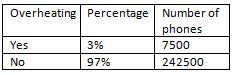
\includegraphics[width=0.35\linewidth,keepaspectratio]{pval1}
\end{center}

Now you have to take a decision whether you will recall the phone from the market or not.


\end{frame}

%%%%%%%%%%%%%%%%%%%%%%%%%%%%%%%%%%%%%%%%%%%%%%%%%%%%%%%%%%%
\begin{frame}[fragile]\frametitle{Level of Significance: p-value: Example}
Hypothesis: Set up null hypothesis and alternate hypothesis first
\begin{itemize}
\item Null hypothesis (H0):= Overheating of phones are as expected and due the some random events which was observed during the production process.
\item Alternate hypothesis (H1):= Overheating of the phones are not due to some random events. There must be some strong reason behind the overheating.
\item If p value is large you accept null hypothesis.
\item If p value is small you fail to accept null hypothesis. You believe that the alternate hypothesis is somewhat acceptable. Your test is statistically significant.
\end{itemize}



\end{frame}

%%%%%%%%%%%%%%%%%%%%%%%%%%%%%%%%%%%%%%%%%%%%%%%%%%%%%%%%%%%
\begin{frame}[fragile]\frametitle{Level of Significance: p-value: Example}
Data: Scenario 1:
\begin{center}
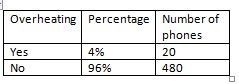
\includegraphics[width=0.35\linewidth,keepaspectratio]{pval2}
\end{center}

Data: Scenario 2:
\begin{center}
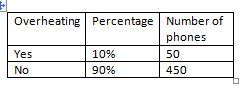
\includegraphics[width=0.35\linewidth,keepaspectratio]{pval3}
\end{center}

The sample size n = 500.

m = 2. (Number of categorical values (Here they are Overheating \& Non-overheating OR Yes \& No))


\end{frame}

%%%%%%%%%%%%%%%%%%%%%%%%%%%%%%%%%%%%%%%%%%%%%%%%%%%%%%%%%%%
\begin{frame}[fragile]\frametitle{Level of Significance: p-value: Example}
Experiments and Results: let’s set the confidence interval first and know about the types of error.

\begin{itemize}
\item H1 Error: - We reject null hypothesis even though it is true. (In our example, even after observing that the overheating of phones happen due to random events we still reject null hypothesis and assume that the overheating happens due to some manufacturing issue.)

\item H2 Error: - We retain null hypothesis even though it is false. (In our example, even after observing that the overheating of phones happen due to some manufacturing issue we still accept null hypothesis and assume that the overheating happens due to random events.)

\end{itemize}

\end{frame}

%%%%%%%%%%%%%%%%%%%%%%%%%%%%%%%%%%%%%%%%%%%%%%%%%%%%%%%%%%%
\begin{frame}[fragile]\frametitle{Level of Significance: p-value: Example}
Experiments and Results: let’s set the confidence interval first and know about the types of error.

\begin{itemize}

\item CI: Confidence interval for our test will be 95\%. This means we are 95\% confident that the test results of our sample will fall 95\% close to the population.

\item $\alpha$ (Significance level) is the probability of H1 error. Here $\alpha = 0.05$.
\end{itemize}

\end{frame}

%%%%%%%%%%%%%%%%%%%%%%%%%%%%%%%%%%%%%%%%%%%%%%%%%%%%%%%%%%%
\begin{frame}[fragile]\frametitle{Level of Significance: p-value: Example}
Scenario 1:

\begin{center}
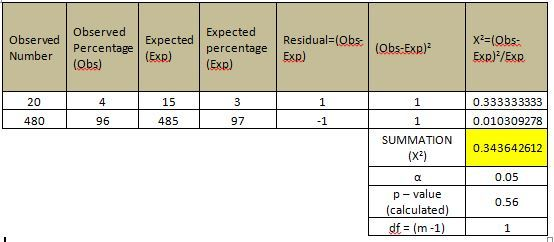
\includegraphics[width=\linewidth,keepaspectratio]{pval4}
\end{center}

\begin{itemize}
\item From the experiment we saw the Chi Square (X2) value is 0.3436 and p-value is 0.56 (calculated).
\item  p-value is greater than the $\alpha$ (=0.05).
\end{itemize}
\end{frame}

%%%%%%%%%%%%%%%%%%%%%%%%%%%%%%%%%%%%%%%%%%%%%%%%%%%%%%%%%%%
\begin{frame}[fragile]\frametitle{Level of Significance: p-value: Example}
Scenario 1:
Search the critical value of X2 from the table. 
\begin{center}
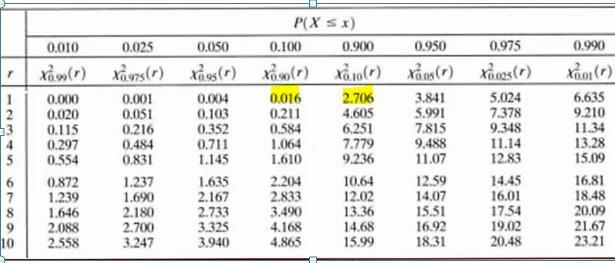
\includegraphics[width=0.8\linewidth,keepaspectratio]{pval5}
\end{center}

\begin{itemize}
\item The next critical value after X2=0.3436 is 2.706 and its corresponding p-value is 0.1. 
\item And our X2 value lies between X20.10 and X20.90. 
\item This means our p-value (though we have already calculated) calculated above is between 0.1 to 0.9 and it is not smaller than 0.05.
\end{itemize}
\end{frame}

%%%%%%%%%%%%%%%%%%%%%%%%%%%%%%%%%%%%%%%%%%%%%%%%%%%%%%%%%%%
\begin{frame}[fragile]\frametitle{Level of Significance: p-value: Example}
Scenario 1:
\begin{itemize}
\item We fail to prove any evidence against null hypothesis. We can’t reject null hypothesis. 
\item This means the number of overheating phones we found from the survey is not significantly different than what we observed during our production process.
\end{itemize}
\end{frame}

%%%%%%%%%%%%%%%%%%%%%%%%%%%%%%%%%%%%%%%%%%%%%%%%%%%%%%%%%%%
\begin{frame}[fragile]\frametitle{Level of Significance: p-value: Example}
Scenario 2:

\begin{center}
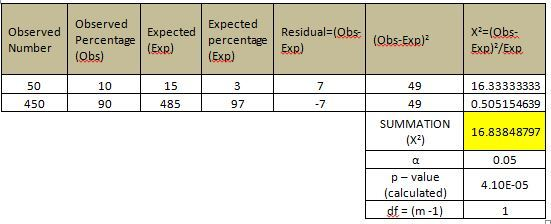
\includegraphics[width=\linewidth,keepaspectratio]{pval6}
\end{center}

\begin{itemize}
\item From the experiment we saw the Chi Square (X2) value is 16.8384 and p –value is 4.10E-05 (calculated).
\item  p-value is smaller than the $\alpha$ (=0.05).
\end{itemize}
\end{frame}

%%%%%%%%%%%%%%%%%%%%%%%%%%%%%%%%%%%%%%%%%%%%%%%%%%%%%%%%%%%
\begin{frame}[fragile]\frametitle{Level of Significance: p-value: Example}
Scenario 2:
We can also search the critical value of X2 from the table. 
\begin{center}
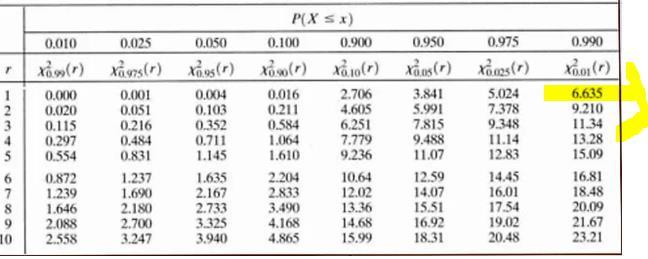
\includegraphics[width=0.8\linewidth,keepaspectratio]{pval7}
\end{center}

\begin{itemize}
\item The next critical value after X2=X2=16.83 is 2.706 and its corresponding p-value is 0.01. 
\item This means our p-value (though we have already calculated) should be less than 0.01 and it is obviously less than 0.05 s well.
\end{itemize}
\end{frame}

%%%%%%%%%%%%%%%%%%%%%%%%%%%%%%%%%%%%%%%%%%%%%%%%%%%%%%%%%%%
\begin{frame}[fragile]\frametitle{Level of Significance: p-value: Example}
Scenario 2:
\begin{itemize}
\item We have to reject null hypothesis. 
\item This means the number of overheating phones we found from the survey is significantly different than what we observed during our production process. And it is not due to some random events.
\end{itemize}
\end{frame}

%%%%%%%%%%%%%%%%%%%%%%%%%%%%%%%%%%%%%%%%%%%%%%%%%%%%%%%%%%%
\begin{frame}[fragile]\frametitle{Level of Significance: p-value: Example}
Outcome of the Problem Statement:
\begin{itemize}
\item For the 1st scenario we will accept the null hypothesis and our phones don’t have any manufacturing problem.
\item For the 2nd scenario we have to check the phones for their manufacturing problem as we have strong evidence against the null hypothesis.
\end{itemize}
\end{frame}


%%%%%%%%%%%%%%%%%%%%%%%%%%%%%%%%%%%%%%%%%%%%%%%%%%%%%%%%%%%
\begin{frame}[fragile]\frametitle{Level of Significance: p-value}
\begin{itemize}


\item P-value:  The  probability  of  getting  test  statistics  as  extreme  as 
observed, under the null hypothesis is P-value. It is the observed 
level of significance. 
 
\item E.g. study placebo group vs new medication group to lower BP.  
\item Mean BP in the treatment group was less by 20mm. Assuming that $H_0$ is true (ie medication has no effect). 
\item If we repeated the study, then the difference in means can go AT MAX to 20mm.
\item P value is how much data disagrees with the Null Hypothesis.
\item  High similarity High P
\item Low p= reject $H_0$, as there is much diff
\item High p= fail to reject $H_0$. no real diff exists.
\item Whether P is low or high is determined by Level of Significations
\end{itemize}
\end{frame}


%%%%%%%%%%%%%%%%%%%%%%%%%%%%%%%%%%%%%%%%%%%%%%%%%%%
\begin{frame}
\frametitle{Graphical: Critical values}
At 95\% $\alpha$
\begin{center}
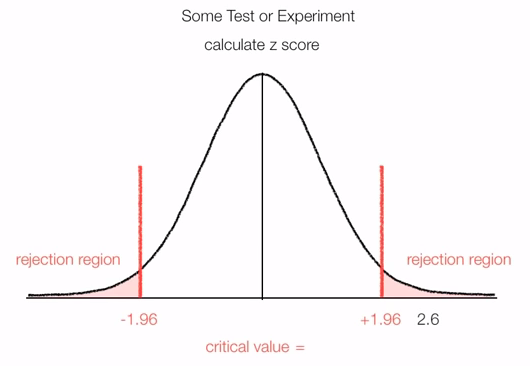
\includegraphics[width=0.45\linewidth,keepaspectratio]{alp1}
\end{center}

\begin{itemize}
\item  Compare if calculate z score of 2.6 is it in rejection region? 
\item Yes, so reject $H_0$
\item Basically, if we are in non-reject region, $H_0$ holds, so no real diff.
\item Only when you cross the band, you are making some diff.
\item That band is controlled by $\alpha$.
\end{itemize}
\end{frame}

%%%%%%%%%%%%%%%%%%%%%%%%%%%%%%%%%%%%%%%%%%%%%%%%%%%
\begin{frame}
\frametitle{Graphical:P Value}
How significant my result is.
\begin{center}
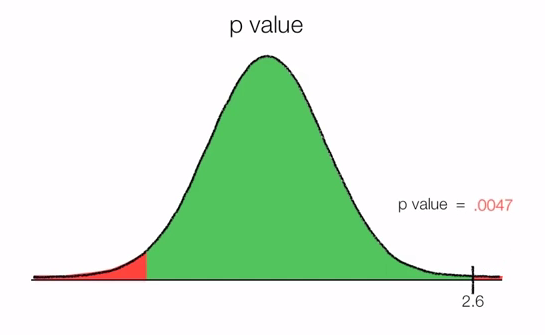
\includegraphics[width=0.5\linewidth,keepaspectratio]{alp2}
\end{center}

\begin{itemize}
\item  In one tail, we have 0.025 area
\item Given z score of 2.6, is above critical value of +1.96.
\item P is area above 2.6
\item It can be calculated from area under normal curve' table to be 0.0047
\item $ p < 0.025$. So, reject $H_0$
\end{itemize}
\end{frame}

%%%%%%%%%%%%%%%%%%%%%%%%%%%%%%%%%%%%%%%%%%%%%%%%%%%%%%%%%%%
\begin{frame}
\begin{center}
{\Large P-Value : Another Example on How to Calculate P Value}
\end{center}
\end{frame}

%%%%%%%%%%%%%%%%%%%%%%%%%%%%%%%%%%%%%%%%%%%%%%%%%%%
\begin{frame}
\frametitle{Introduction (recap)}

\begin{itemize}
\item P value is a statistical measure that helps scientists determine whether their hypotheses are correct.
\item Usually, if the P value of a data set is below a certain pre-determined amount (like, for instance, 0.05), scientists will reject the "null hypothesis" of their experiment - in other words, they'll rule out the hypothesis that the variables of their experiment had no meaningful effect on the results. 
\item Today, p values are usually found on a reference table by first calculating a chi square value.

\end{itemize}
\end{frame}

%%%%%%%%%%%%%%%%%%%%%%%%%%%%%%%%%%%%%%%%%%%%%%%%%%%
\begin{frame}
\frametitle{Expected Results (recap)}

\begin{itemize}
\item Usually, when scientists conduct an experiment and observe the results, they have an idea of what "normal" or "typical" results will look like beforehand. This can be based on past experimental results, trusted sets of observational data, etc.
\item For your experiment, determine your expected results and express them as a number.
\end{itemize}
\end{frame}

%%%%%%%%%%%%%%%%%%%%%%%%%%%%%%%%%%%%%%%%%%%%%%%%%%%
\begin{frame}
\frametitle{Toy Experiment}

\begin{itemize}
\item Let's say prior studies have shown that, nationally, speeding tickets are given more often to red cars than they are to blue cars
\item Let's say the average results nationally show a 2:1 preference for red cars. We want to find out whether or not the police in our town also demonstrate this bias by analyzing speeding tickets given by our town's police. 
\item If we take a random pool of 150 speeding tickets given to either red or blue cars in our town, we would expect 100 to be for red cars and 50 to be for blue cars if our town's police force gives tickets according to the national bias.
\end{itemize}

\begin{center}
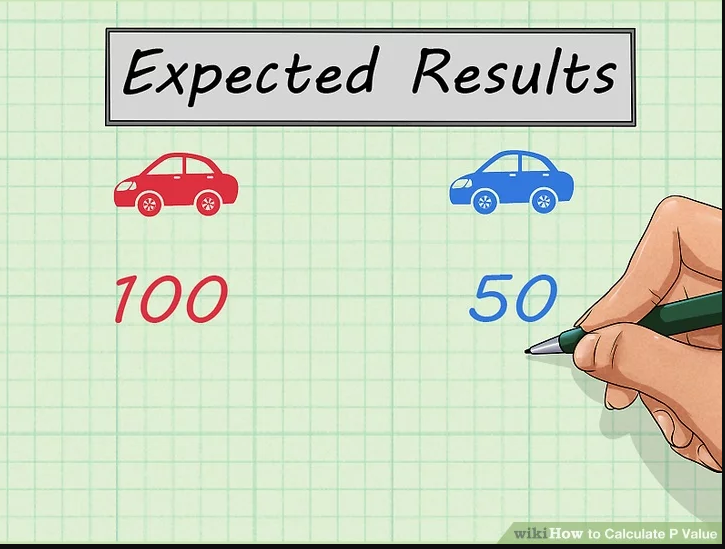
\includegraphics[width=0.5\linewidth,keepaspectratio]{pvalue1}
\end{center}
\end{frame}


%%%%%%%%%%%%%%%%%%%%%%%%%%%%%%%%%%%%%%%%%%%%%%%%%%%
\begin{frame}
\frametitle{Determine your experiment's observed results}
You can conduct your experiment and find your actual (or "observed") values. Again, express these results as numbers. Following were numbers from LOCAL (not national) observations. See if chaning this data source (National to local) had any significant effect.

\begin{center}
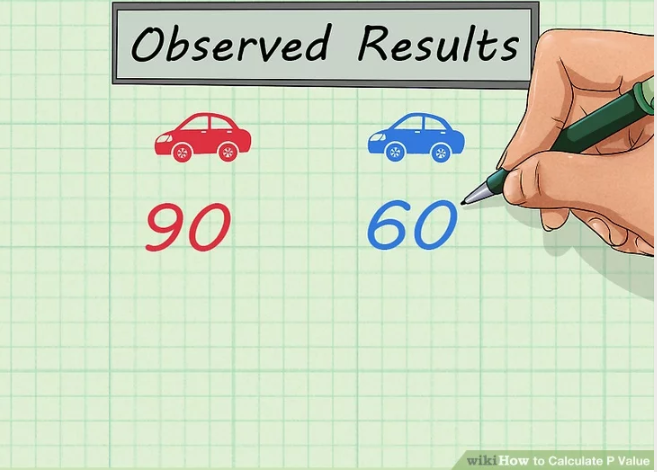
\includegraphics[width=0.5\linewidth,keepaspectratio]{pvalue2}
\end{center}
\end{frame}

%%%%%%%%%%%%%%%%%%%%%%%%%%%%%%%%%%%%%%%%%%%%%%%%%%%
\begin{frame}
\frametitle{Experiment's observed results}
\begin{itemize}
\item The observed results differ from this expected results, two possibilities are possible: either this happened by chance, or our experimental variables caused the difference. 
\item The purpose of finding a p-value is to determine whether the observed results differ from the expected results to such a degree that the "null hypothesis" - the hypothesis that there is no relationship between the experimental variable(s) and the observed results - is unlikely enough to reject. It did not happen by chance.
\item Are our local police as biased as the national average suggests, and we're just observing a chance variation? A p value will help us determine this.

\end{itemize}

\end{frame}

%%%%%%%%%%%%%%%%%%%%%%%%%%%%%%%%%%%%%%%%%%%%%%%%%%%
\begin{frame}
\frametitle{Determine your experiment's degrees of freedom}
\begin{itemize}
\item Degrees of freedom are a measure the amount of variability involved in the research, which is determined by the number of categories you are examining. The equation for degrees of freedom is Degrees of freedom = n-1, where "n" is the number of categories or variables being analyzed in your experiment.
\item Example: Our experiment has two categories of results: one for red cars and one for blue cars. Thus, in our experiment, we have 2-1 = 1 degree of freedom. If we had compared red, blue, and green cars, we would have 2 degrees of freedom, and so on.
\end{itemize}

\begin{center}
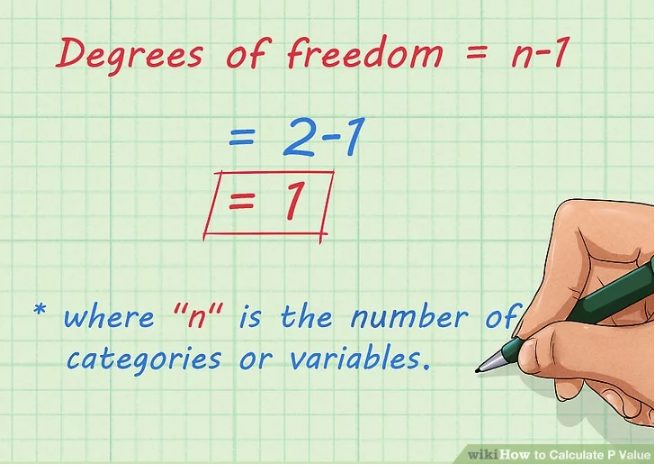
\includegraphics[width=0.5\linewidth,keepaspectratio]{pvalue3}
\end{center}

\end{frame}

%%%%%%%%%%%%%%%%%%%%%%%%%%%%%%%%%%%%%%%%%%%%%%%%%%%
\begin{frame}
\frametitle{Compare expected results to observed results with chi square}
\begin{itemize}
\item Chi square(written "x2") is a numerical value that measures the difference between an experiment's expected and observed values. 
\item The equation for chi square is: $x2 = \sum((o-e)2/e)$, where ``o'' is the observed value and ``e'' is the expected value
\begin{itemize}
\item $x2 = ((90-100)2/100) + (60-50)2/50)$
\item $x2 = ((-10)2/100) + (10)2/50)$
\item $x2 = (100/100) + (100/50) = 1 + 2 = 3$
\end{itemize}

\end{itemize}

\begin{center}
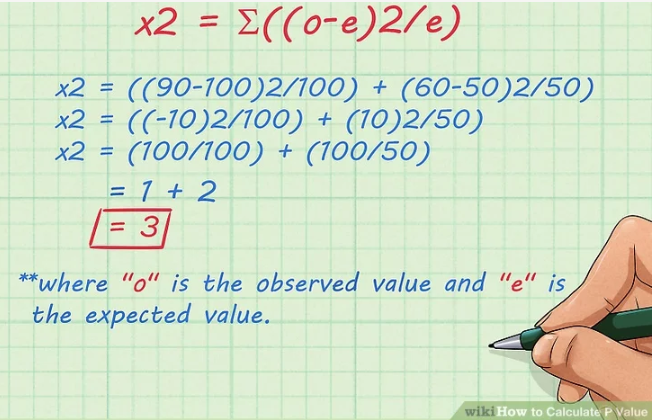
\includegraphics[width=0.5\linewidth,keepaspectratio]{pvalue4}
\end{center}

\end{frame}

%%%%%%%%%%%%%%%%%%%%%%%%%%%%%%%%%%%%%%%%%%%%%%%%%%%
\begin{frame}
\frametitle{Choose a significance level}
\begin{itemize}
\item Basically, the significance level is a measure of how certain we want to be about our results - low significance values correspond to a low probability that the experimental results happened by chance, and vice versa.
\item By convention, scientists usually set the significance value for their experiments at 0.05, or 5 percent.
\item This means that experimental results that meet this significance level have, at most, a 5\% chance of being reproduced in a random sampling process

\end{itemize}

\end{frame}

%%%%%%%%%%%%%%%%%%%%%%%%%%%%%%%%%%%%%%%%%%%%%%%%%%%
\begin{frame}
\frametitle{Chi square table}

\begin{center}
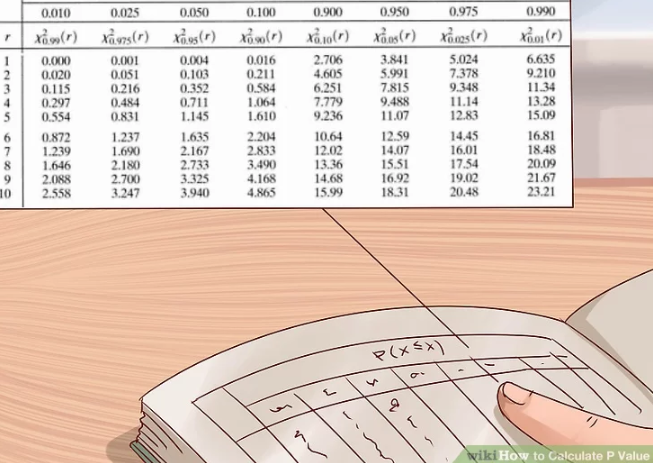
\includegraphics[width=0.9\linewidth,keepaspectratio]{pvalue5}
\end{center}

\end{frame}

%%%%%%%%%%%%%%%%%%%%%%%%%%%%%%%%%%%%%%%%%%%%%%%%%%%
\begin{frame}
\frametitle{Use a chi square distribution table to approximate your p-value}
\begin{itemize}
\item Use these tables by first finding your degrees of freedom, then reading that row across from the left to the right until you find the first value bigger than your chi square value. 
\item Look at the corresponding p value at the top of the column - your p value is between this value and the next-largest value (the one immediately to the left of it.)
\item We'll go from left to right along this row until we find a value higher than 3 - our chi square value. The first one we encounter is 3.84. Looking to the top of this column, we see that the corresponding p value is 0.05. 
\item This means that our p value is between 0.05 and 0.1 (the next-biggest p value on the table).
\end{itemize}

\end{frame}

%%%%%%%%%%%%%%%%%%%%%%%%%%%%%%%%%%%%%%%%%%%%%%%%%%%
\begin{frame}
\frametitle{Decide whether to reject or keep your null hypothesis}
\begin{itemize}
\item Our p value is between 0.05 and 0.1 . It is not smaller than 0.05, so, unfortunately, we can't reject our null hypothesis. 
\item This means that we didn't reach the criterion we decided upon to be able to say that our town's police give tickets to red and blue cars at a rate that's significantly different than the national average.
\item In other words, random sampling from the national data would produce a result 10 tickets off from the national average 5-10\% of the time.

\item Since we were looking for this percentage to be less than 5\%, we can't say that we're sure our town's police are less biased towards red cars.
\end{itemize}

\end{frame}

%%%%%%%%%%%%%%%%%%%%%%%%%%%%%%%%%%%%%%%%%%%%%%%%%%%%%%%%%%%
\begin{frame}
\begin{center}
{\Large Hypothesis Testing}
\end{center}
\end{frame}

%%%%%%%%%%%%%%%%%%%%%%%%%%%%%%%%%%%%%%%%%%%%%%%%%%%%%%%%%%%
\begin{frame}[fragile]\frametitle{Statistical Hypothesis Testing}
\begin{itemize}
\item t-test = compares 1/2 numerical groups
\item ANOVA = compares $> 2$ numerical groups
\item Chi-square test  = compares categorical variables
\end{itemize}
\end{frame}

%%%%%%%%%%%%%%%%%%%%%%%%%%%%%%%%%%%%%%%%%%%%%%%%%%%%%%%%%%%
\begin{frame}
\begin{center}
{\Large t-Test}
\end{center}
\end{frame}

%%%%%%%%%%%%%%%%%%%%%%%%%%%%%%%%%%%%%%%%%%%%%%%%%%%%%%%%%%%%%%%%%%%%%%%%
\begin{frame}[fragile]\frametitle{t-Test}

	\begin{itemize}
	
	\item There are two types of t-tests: paired and unpaired.
	\item Paired t-tests are used when you have `before' and `after' measurements from the same subjects. E.g body temperature before and after medicine.
	\item Unpaired: you are comparing height data for two groups. 
	\item Subcategories of Unpaired t-tests:
	\begin{itemize}
	\item Assumes that variations with both groups are same.
	\item Does NOT Assume that variations with both groups are same.
	\end{itemize}
	\item Another classification: 1-tail or 2-tails t-tests
	\item In case of comparing heights of two groups, the 2-tail t-test will evaluate of group A is Higher than B as well as Shorter than B, ie at both ends.
	\item It is used when you already know which direction has to be compared, higher or lower.
	\end{itemize}
  
 
\tiny{(Ref: StatQuest: Which t test to use? - Josh Starmer )}
\end{frame}

%%%%%%%%%%%%%%%%%%%%%%%%%%%%%%%%%%%%%%%%%%%%%%%%%%%%%%%%%%%%%%%%%%%%%%%%
\begin{frame}[fragile]\frametitle{1 vs 2 tailed t-Tests}
Example: a clinical trial is done on 6 patients to find effect of a new drug.


	\begin{itemize}
	\item Data shows that with new drug, results are much better (more red dots on left)
	\item The red dot in the middle is a bit problematic.
	\item After doing stats, you get p-value of 0.03 for 1 tail t test. 
	\item 0.03 is smaller than threshold of 0.05 (CI). Meaning this new drug is significantly different. Its mean result is far away from other means found during existing treatments.
	\item 2-tailed gives p-value of 0.06. Not good.
	\item Which p-value to use?
	\end{itemize}

      \begin{center}
      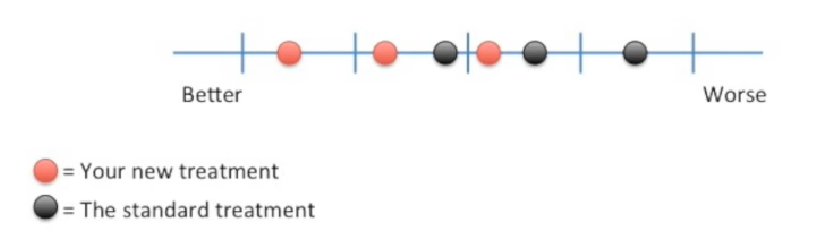
\includegraphics[width=\linewidth,keepaspectratio]{statq41}
	  	\end{center}

\tiny{(Ref: StatQuest: One or Two Tailed P-Values - Josh Starmer )}
\end{frame}

%%%%%%%%%%%%%%%%%%%%%%%%%%%%%%%%%%%%%%%%%%%%%%%%%%%%%%%%%%%%%%%%%%%%%%%%
\begin{frame}[fragile]\frametitle{1 vs 2 tailed t-Tests}
Example: a clinical trial is done on 6 patients to find effect of a new drug.


	\begin{itemize}
	\item 1 tailed p value tests the hypothesis that your new drug is better than the existing drug. Whereas,
	\item 2 tailed p-value tests whether the new drug is better , worse or not significantly different.
	\item 1 tailed p value is smaller because it does not distinguish between ``worse'' or ``not significantly different''.
	\item AS we wish to know if the new drug was worse than the existing treatment, we should use 2 tailed p value test.
	\end{itemize}

      \begin{center}
      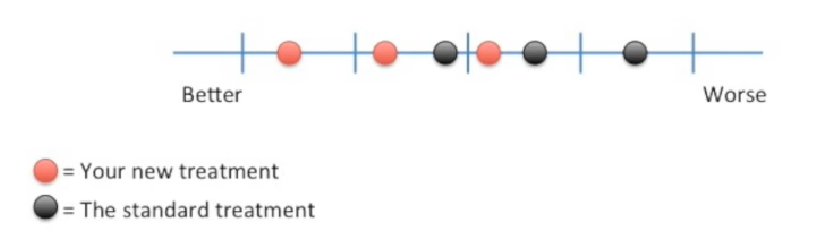
\includegraphics[width=\linewidth,keepaspectratio]{statq41}
	  	\end{center}

\tiny{(Ref: StatQuest: One or Two Tailed P-Values - Josh Starmer )}
\end{frame}


%%%%%%%%%%%%%%%%%%%%%%%%%%%%%%%%%%%%%%%%%%%%%%%%%%%%%%%%%%%
\begin{frame}[fragile]\frametitle{t-tests}
\begin{itemize}
\item One sample hypothesis testing
\begin{itemize}
\item We are given population $\sigma$: use z distribution, z-test
\item We are Not given population $\sigma$, need to estimate it: t-distribution, t-test
\end{itemize}
\item Two sample t-test 
%\item Paired t-test 
\end{itemize}
\end{frame}

%%%%%%%%%%%%%%%%%%%%%%%%%%%%%%%%%%%%%%%%%%%%%%%%%%%
\begin{frame}
\frametitle{Z distribution}
Same as Sampling distribution
\begin{center}
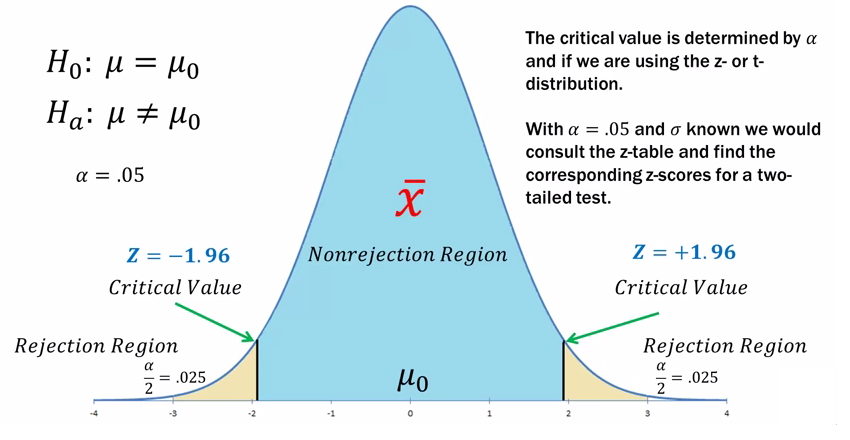
\includegraphics[width=\linewidth,keepaspectratio]{zdist}
\end{center}
\end{frame}

%%%%%%%%%%%%%%%%%%%%%%%%%%%%%%%%%%%%%%%%%%%%%%%%%%%
\begin{frame}
\frametitle{t distribution}
Every t distribution is unique and is specific to sample size. For n=20, look at t table with degrees of freedom 20-1=19
\begin{center}
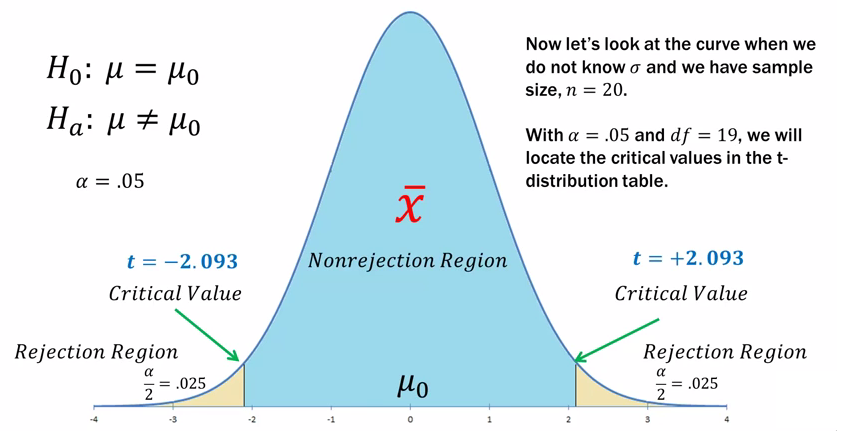
\includegraphics[width=0.8\linewidth,keepaspectratio]{tdist}
\end{center}
Range is a bit more than Z dist. Like pushing it down from top!!
\end{frame}

%%%%%%%%%%%%%%%%%%%%%%%%%%%%%%%%%%%%%%%%%%%%%%%%%%%%%%%%%%%
\begin{frame}[fragile]\frametitle{One Sample t-test}
\begin{itemize}
\item Objective: Test if hypothesized population mean matches with the actual population mean.
\item $\mu_0$ is hypothesized population mean
\item $\mu$ is the true/actual population mean
\item Method: Test using sample means and confidence interval
\end{itemize}
\end{frame}

%%%%%%%%%%%%%%%%%%%%%%%%%%%%%%%%%%%%%%%%%%%%%%%%%%%%%%%%%%%
\begin{frame}[fragile]\frametitle{One Sample t-test}
\begin{itemize}
\item When?: To test whether a given sample is coming from a population whose mean is specified value
$$
t = \frac{\bar{x} - \mu_0}{s /\sqrt{n}}
$$
\item $\bar{x}$: sample mean of n observations
\item $s$: sample std deviation of n observations
\item $\mu_0$: hypothesized population mean
\item $H_0: \bar{x} = \mu_0$
\item $H_1: \bar{x} \neq \mu_0$
\end{itemize}
\end{frame}

%%%%%%%%%%%%%%%%%%%%%%%%%%%%%%%%%%%%%%%%%%%%%%%%%%%%%%%%%%%
\begin{frame}[fragile]\frametitle{One Sample t-test}
\begin{itemize}
\item t value computed is similar to z score.
\item Shows how many std deviations you are away from mean.
\item With the given t score, in the t table find the location on graph
\item Looking at cut off boundaries, are you landing in the non rejection region or the rejection region?
\end{itemize}
\end{frame}

%%%%%%%%%%%%%%%%%%%%%%%%%%%%%%%%%%%%%%%%%%%%%%%%%%%%%%%%%%%
\begin{frame}[fragile]\frametitle{Example: One Sample t-test}
\begin{itemize}
\item New tyres launched are claim to have life of 40000 km.
\item A retailer wants to test this claim.
\item He has taken random sample of 8 tyres.
\item He is testing life of the tyres under normal condition.
\end{itemize}
\end{frame}

%%%%%%%%%%%%%%%%%%%%%%%%%%%%%%%%%%%%%%%%%%%%%%%%%%%%%%%%%%%
\begin{frame}[fragile]\frametitle{Example: One Sample t-test}
\begin{itemize}
\item We don't know population std dev. So t test.
\item $H_0; \mu_0 = 40000$ 
\item $H_1; \mu_0 \ne 40000$ 
\item Lets take $\alpha = 0.05$
\item $df = n -1 = 8 - 1 = 7$
\end{itemize}
\end{frame}

%%%%%%%%%%%%%%%%%%%%%%%%%%%%%%%%%%%%%%%%%%%%%%%%%%%%%%%%%%%
\begin{frame}[fragile]\frametitle{Example: One Sample t-test}
\begin{center}
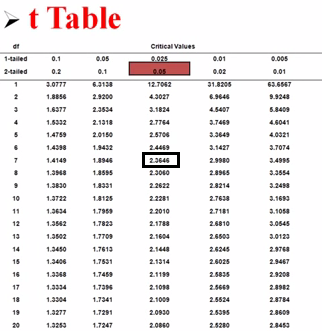
\includegraphics[width=0.5\linewidth,keepaspectratio]{ttble}
\end{center}
\begin{itemize}
\item Critical boundary-value = 2.3646
\item If t false below -2.3646 or above 2.3646, then reject $H_0$.
\end{itemize}
\end{frame}



%%%%%%%%%%%%%%%%%%%%%%%%%%%%%%%%%%%%%%%%%%%%%%%%%%%%%%%%%%%
\begin{frame}[fragile]\frametitle{Example: One Sample t-test}

\begin{itemize}
\item  His findings below:
 
\begin{tabular}{l|l}
Sr	&Km\\ \hline
1 & 35000\\
2 & 38000\\
3 & 42000\\
4 & 41000\\
5 & 39000\\
6 & 41500\\
7 & 43000\\
8 & 38500\\
\end{tabular}
\item Given goal mean $\mu_0 = 40000$
\item $n = 8$
\item Calculate sample mean $\bar{x}$, it comes to $39750$
\item Calculate $s$, it comes to $2618.615$
\item $df = n -1 = 7$
\end{itemize}
\end{frame}

%%%%%%%%%%%%%%%%%%%%%%%%%%%%%%%%%%%%%%%%%%%%%%%%%%%%%%%%%%%
\begin{frame}[fragile]\frametitle{Example: One Sample t-test}

\begin{itemize}
\item $t = \frac{\bar{x} - \mu_0}{s /\sqrt{n}} = \frac{39750 - 40000}{2618.615 /\sqrt{8}} = \frac{-250}{925.82} = - 0.27$
\item It is right of negative boundary and left of positive boundary, 
\item So, in valid region.
\item So, cannot reject $H_0$. 
\item So, no difference. 
\item Sample mean is same as given mean.
\end{itemize}
\end{frame}


%%%%%%%%%%%%%%%%%%%%%%%%%%%%%%%%%%%%%%%%%%%%%%%%%%%%%%%%%%%
\begin{frame}[fragile]\frametitle{Two Samples t-test}
\begin{itemize}
\item When?: To test whether given two samples are coming from a population
$$
t = \frac{\bar{x_1} - \bar{x_2}}{s_p /\sqrt{\frac{1}{n_1} + \frac{1}{n_2}}}
$$
\item $\bar{x_1}$: sample mean of $n_1$ observations
\item $\bar{x_2}$: sample mean of $n_2$ observations
\item $s_p$: Pooled std deviation of two samples
\item $\mu_0$: specified population mean
\item $H_0: \bar{x_1} = \bar{x_2}$
\item $H_1: \bar{x_1} \neq \bar{x_2}$
\end{itemize}
\end{frame}

%%%%%%%%%%%%%%%%%%%%%%%%%%%%%%%%%%%%%%%%%%%%%%%%%%%%%%%%%%%
\begin{frame}[fragile]\frametitle{Example: Two Sample t-test}
\begin{itemize}
\item Is there any appreciable difference of IQs of Males and Females?
\item $H_0: \bar{x_{male}} = \bar{x_{female}}$
\item $H_1: \bar{x_{male}} \neq \bar{x_{female}}$
\item Lets take $\alpha = 0.05$
\item $n_m = n_f = 18; n= 36$
\item $ \bar{x_{male}} = 98.9$
\item $ \bar{x_{female}} = 102.4 $
\item $s = 12$; same for both
\end{itemize}
\end{frame}

%%%%%%%%%%%%%%%%%%%%%%%%%%%%%%%%%%%%%%%%%%%%%%%%%%%%%%%%%%%
\begin{frame}[fragile]\frametitle{Example: Two Sample t-test}
\begin{itemize}
\item Finding critical values value for t at $1 - \alpha/2$ for two tail test and  $df = n -1 = 35$ = 2.030
\item $t = \frac{\bar{x_{female}} - \bar{x_{male}}}{s_p /\sqrt{\frac{1}{n_f} + \frac{1}{n_m}}}$
\item $ = \frac{102.4- 98.9}{12/ \sqrt{1/18 + 1/18}} = 0.097$
\item Lies in acceptable region.
\item Can not reject $H_0$
\item No diff in IQs.
\end{itemize}
\end{frame}

%%%%%%%%%%%%%%%%%%%%%%%%%%%%%%%%%%%%%%%%%%%%%%%%%%%
\begin{frame}[fragile]\frametitle{Two Samples t-test}
What is t-test?
\begin{itemize}
\item Compares two averages (means) and tells you if they are different from each other. 
\item Tells you how significant the differences are
\item It lets you know if those differences could have happened by chance.
\end{itemize}
\end{frame}

%%%%%%%%%%%%%%%%%%%%%%%%%%%%%%%%%%%%%%%%%%%%%%%%%%%
\begin{frame}[fragile]\frametitle{Two Samples t-test}
What is t-test?
\begin{itemize}
\item The t score is a ratio between the difference between two groups and the difference within the groups.
\item A large t-score tells you that the groups are different.
\item A small t-score tells you that the groups are similar.
\item  The bigger the t-value, the more likely it is that the results are repeatable.
\end{itemize}
\end{frame}

%%%%%%%%%%%%%%%%%%%%%%%%%%%%%%%%%%%%%%%%%%%%%%%%%%%
\begin{frame}[fragile]\frametitle{Two Samples t-test}
\begin{itemize}
\item Every t-value has a p-value to go with it. A p-value is the probability that the results from your sample data occurred by chance. 
\item a p-value of .01 means there is only a 1\% probability that the results from an experiment happened by chance.
\end{itemize}
\end{frame}

%%%%%%%%%%%%%%%%%%%%%%%%%%%%%%%%%%%%%%%%%%%%%%%%%%%
\begin{frame}[fragile]\frametitle{Two Samples t-test}
Types of t-tests?
\begin{itemize}
\item  An Independent Samples t-test compares the means for two groups.
\item  A Paired sample t-test compares means from the same group at different times (say, one year apart).
\item  A One sample t-test tests the mean of a single group against a known mean.
\end{itemize}
\end{frame}

%%%%%%%%%%%%%%%%%%%%%%%%%%%%%%%%%%%%%%%%%%%%%%%%%%%
\begin{frame}[fragile]\frametitle{Two Samples t-test}
Example: to test whether the height of men in the population is different from height of women in general.

Steps:
\begin{itemize}
\item  Determine a null and alternate hypothesis.
\begin{itemize}
\item  Null-Hypothesis: no statistically significant difference, height of men and women are the same
\item  Alternate-Hypothesis: statistically significant difference, height of men and women are different
\end{itemize}
\item Collect sample data. Twos sets: men and women. Generally sizes should be same, but can be diferent, $n_x$ and $n_y$
\end{itemize}
\end{frame} 
%%%%%%%%%%%%%%%%%%%%%%%%%%%%%%%%%%%%%%%%%%%%%%%%%%%
\begin{frame}[fragile]\frametitle{Two Samples t-test}
Steps (cont.):
\begin{itemize}
\item  Determine a confidence interval and degrees of freedom
\item $\alpha$ of 0.005 is 95\% confidence that the conclusion of this test will be valid
\item The degree of freedom $df = n_x + n_y - 2$
\item Calculate the t-statistic

\begin{center}
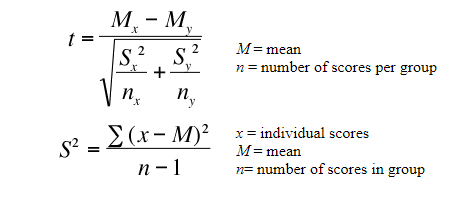
\includegraphics[width=0.8\linewidth,keepaspectratio]{ttestform}
\end{center}
\end{itemize}
\end{frame} 


%%%%%%%%%%%%%%%%%%%%%%%%%%%%%%%%%%%%%%%%%%%%%%%%%%%
\begin{frame}[fragile]\frametitle{Two Samples t-test}
Steps (cont.):
\begin{itemize}
\item  Calculate the critical t-value from the t distribution
\begin{center}
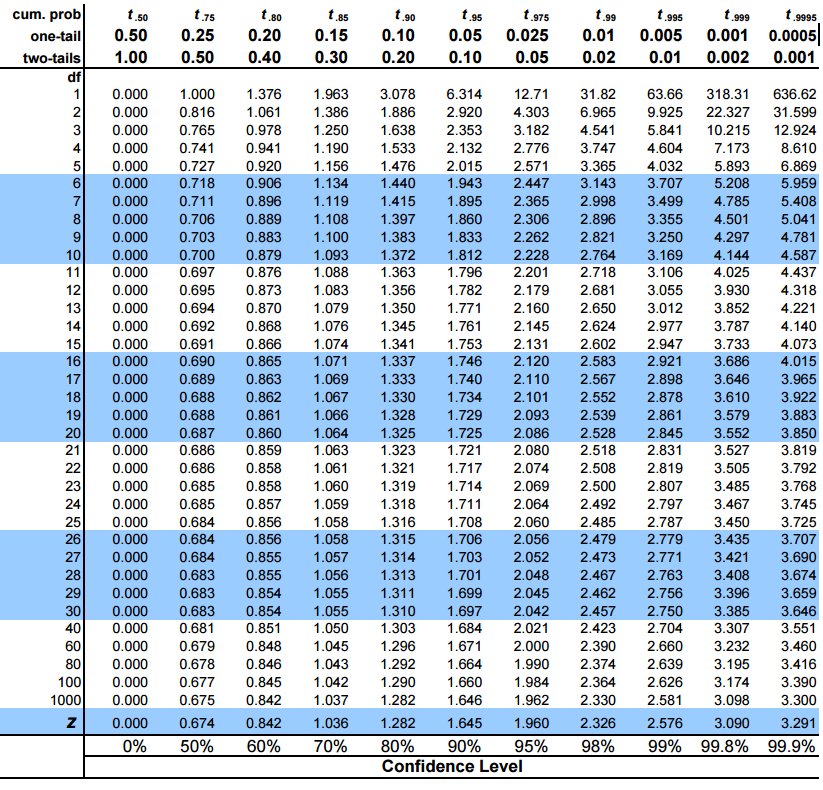
\includegraphics[width=0.6\linewidth,keepaspectratio]{ttesttab}
\end{center}
\item or call ready Python function
\end{itemize}
\end{frame} 


%%%%%%%%%%%%%%%%%%%%%%%%%%%%%%%%%%%%%%%%%%%%%%%%%%%
\begin{frame}[fragile]\frametitle{Two Samples t-test}
Generate data
\begin{lstlisting}
#Sample Size
N = 10
#Gaussian distributed data with mean = 2 and var = 1
a = np.random.randn(N) + 2
#Gaussian distributed data with with mean = 0 and var = 1
b = np.random.randn(N)
\end{lstlisting}
\end{frame}


%%%%%%%%%%%%%%%%%%%%%%%%%%%%%%%%%%%%%%%%%%%%%%%%%%%
\begin{frame}[fragile]\frametitle{Two Samples t-test}
\begin{lstlisting}
#Calculate the variance to get the standard deviation
#For unbiased max likelihood estimate we have to divide the var by N-1, and therefore the parameter ddof = 1

var_a = a.var(ddof=1)
var_b = b.var(ddof=1)

#std deviation
s = np.sqrt((var_a + var_b)/2)
\end{lstlisting}
\end{frame}


%%%%%%%%%%%%%%%%%%%%%%%%%%%%%%%%%%%%%%%%%%%%%%%%%%%
\begin{frame}[fragile]\frametitle{Two Samples t-test}
\begin{lstlisting}
## Calculate the t-statistics
t = (a.mean() - b.mean())/(s*np.sqrt(2/N))
## Compare with the critical t-value
#Degrees of freedom
df = 2*N - 2
#p-value after comparison with the t 
p = 1 - stats.t.cdf(t,df=df)
#Note that we multiply the p value by 2 because its a twp tail t-test

## Cross Checking with the internal scipy function
t2, p2 = stats.ttest_ind(a,b)
\end{lstlisting}
\end{frame} 


%%%%%%%%%%%%%%%%%%%%%%%%%%%%%%%%%%%%%%%%%%%%%%%%%%%%%%%%%%%
\begin{frame}[fragile]\frametitle{Paired t-test}
\begin{itemize}
\item When?: To check, effectiveness of a new treatment, a new method 
employed 
\item  observations on  every  unit  are  made  before  and  after  applying  the  treatment  or 
method.  
\item Hence  if  treatment  or  method  is  effective,  there  will  be 
significant  difference  in  observations  before  applying  it  and  after 
applying it. 
$$
t = \frac{\bar{x_D} - \mu_0}{\sigma_D /\sqrt{n}}
$$
\item $\bar{x_D}$: mean difference of n paired obsrevations
\item $\sigma_D$:  std deviation of difference of n paired obsrevations obsrevations
\item $\mu_0$: mean difference of n paired observations under $H_0$
\item $H_0: $ Mean of samples before and after treatment is same. 
\item $H_1:$ Mean of samples before and after treatment is not same.
\end{itemize}
\end{frame}


%%%%%%%%%%%%%%%%%%%%%%%%%%%%%%%%%%%%%%%%%%%%%%%%%%%%%%%%%%%
\begin{frame}[fragile]\frametitle{Chi-Square test}
\begin{itemize}
\item When?: To test whether any 
two  categorical variables  are  associated  with  each  other  or  they  are 
independent  of  each  other,
$$
x^2= \sum \frac{(O_i - E_i)^2}{E_i}
$$
\item $O_i:$ Observed frequency of ith variable
\item $E_i:$ Expected frequency of ith variable
\item $H_0: $ Two variable are independent of each other. 
\item $H_1:$ Two variable are not independent of each other. 
\end{itemize}
\end{frame}

%%%%%%%%%%%%%%%%%%%%%%%%%%%%%%%%%%%%%%%%%%%%%%%%%%%%%%%%%%%
\begin{frame}[fragile]\frametitle{F test}
\begin{itemize}
\item When?: to  know 
whether  these  two  sample  have  same  population  variance
$$
F = \frac{s_1^2}{s_2^2}
$$
\item $S_1^2$ Sample variance of first sample of size $n_1$
\item $S_2^2$ Sample variance of second sample of size $n_2$
\item $H_0: $ Variance ratio is one
\item $H_1:$ Variance ratio not equal to one
\end{itemize}
\end{frame}


%%%%%%%%%%%%%%%%%%%%%%%%%%%%%%%%%%%%%%%%%%%%%%%%%%%%%%%%%%%%%%%%%%%%%%%%%%%%%%%%%%
\begin{frame}[fragile]\frametitle{}
\begin{center}
{\Large Anova}
\end{center}
\end{frame}

%%%%%%%%%%%%%%%%%%%%%%%%%%%%%%%%%%%%%%%%%%%%%%%%%%%%%%%%%%%
\begin{frame}[fragile]\frametitle{Analysis of Variance (ANOVA)}
The difference between ANOVA and the t tests is that ANOVA can 
be  used  in  situations  where  there  are  two  or  more  means  being 
compared, whereas the t tests are limited to situations where only 
two means are involved. 
\end{frame}

%%%%%%%%%%%%%%%%%%%%%%%%%%%%%%%%%%%%%%%%%%%%%%%%%%%%%%%%%%%
\begin{frame}[fragile]\frametitle{Analysis of Variance (ANOVA)}
\begin{center}
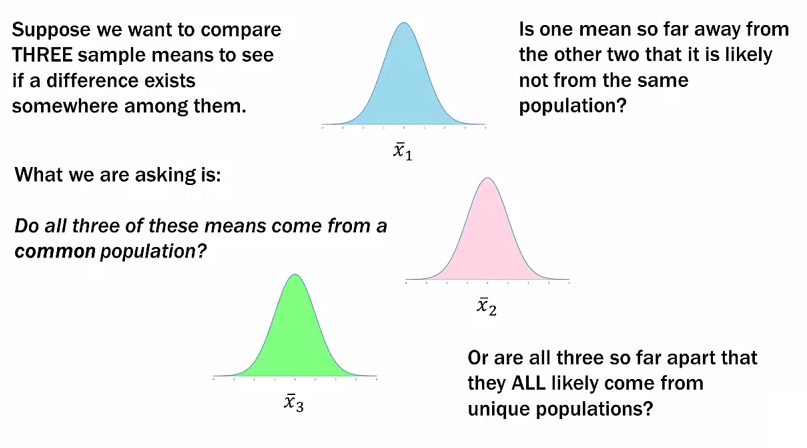
\includegraphics[width=\linewidth,keepaspectratio]{anv1}
\end{center}
Finding DISTANCE between means

\tiny{(Reference: Statistics 101 - Brandon Foltz)}

\end{frame}

%%%%%%%%%%%%%%%%%%%%%%%%%%%%%%%%%%%%%%%%%%%%%%%%%%%%%%%%%%%
\begin{frame}[fragile]\frametitle{Analysis of Variance (ANOVA)}
Combine all data points from all 3 samples. Draw its distribution. Then compare of each with the combined one.
\begin{center}
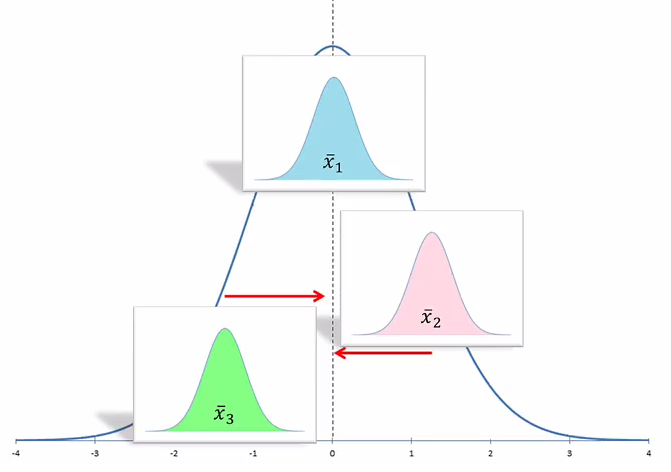
\includegraphics[width=0.7\linewidth,keepaspectratio]{anv2}
\end{center}
$\bar{x}_1$ bang on combined mean, rest are a bit away.
\end{frame}

%%%%%%%%%%%%%%%%%%%%%%%%%%%%%%%%%%%%%%%%%%%%%%%%%%%%%%%%%%%
\begin{frame}[fragile]\frametitle{Analysis of Variance (ANOVA)}
New example: where $\bar{x}_3$  is far away. So not part of combined population. Outlier.

\begin{center}
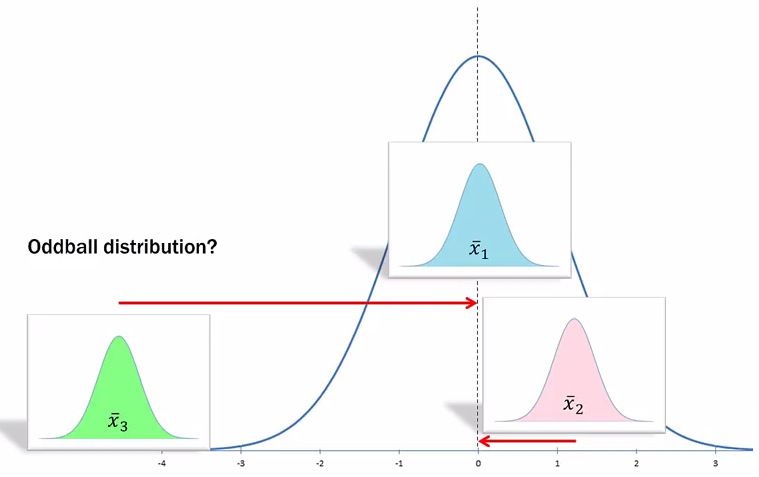
\includegraphics[width=0.8\linewidth,keepaspectratio]{anv3}
\end{center}

\end{frame}

%%%%%%%%%%%%%%%%%%%%%%%%%%%%%%%%%%%%%%%%%%%%%%%%%%%%%%%%%%%
\begin{frame}[fragile]\frametitle{Analysis of Variance (ANOVA)}
New example: where both $\bar{x}_2$ and $\bar{x}_3$  are far away. All three are their OWN populations.

\begin{center}
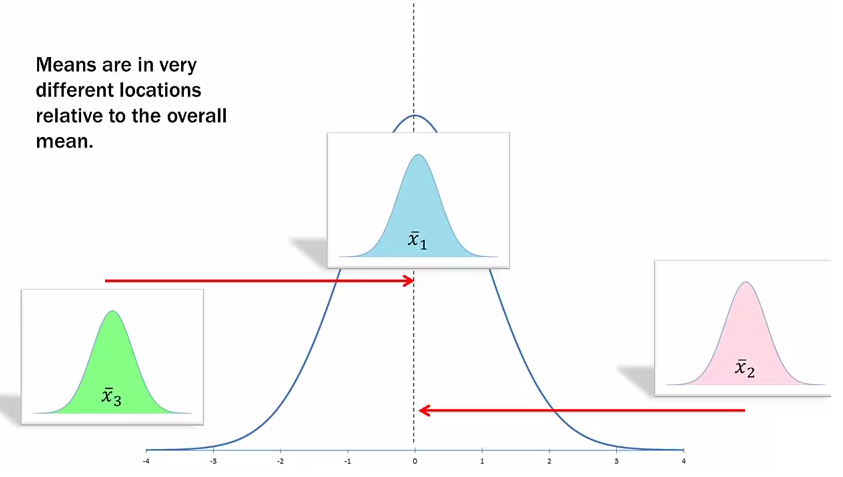
\includegraphics[width=0.8\linewidth,keepaspectratio]{anv4}
\end{center}

\end{frame}

%%%%%%%%%%%%%%%%%%%%%%%%%%%%%%%%%%%%%%%%%%%%%%%%%%%%%%%%%%%
\begin{frame}[fragile]\frametitle{Analysis of Variance (ANOVA)}
\begin{center}
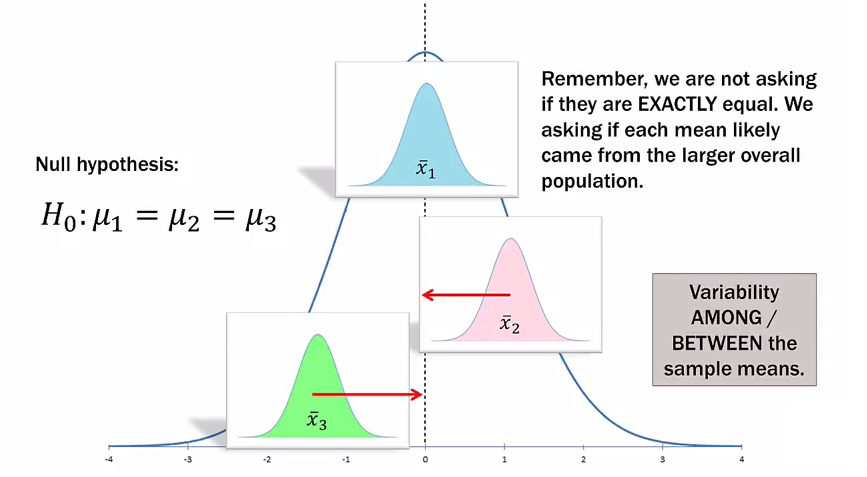
\includegraphics[width=0.8\linewidth,keepaspectratio]{anv5}
\end{center}
Variability is between means.
\end{frame}

%%%%%%%%%%%%%%%%%%%%%%%%%%%%%%%%%%%%%%%%%%%%%%%%%%%%%%%%%%%
\begin{frame}[fragile]\frametitle{Analysis of Variance (ANOVA)}
Pair wise t tests
\begin{center}
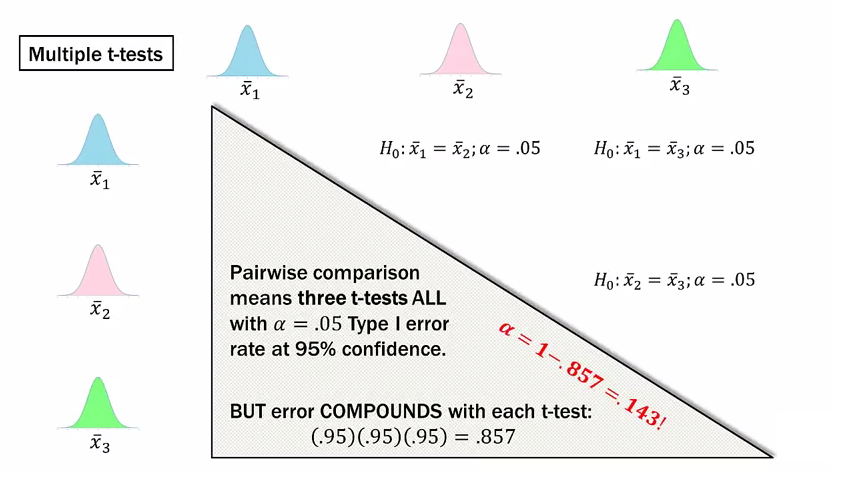
\includegraphics[width=0.8\linewidth,keepaspectratio]{anv6}
\end{center}
Combined error rate went from 5\% to 14.3\%. So we do not conduct multiple t tests.
\end{frame}

%%%%%%%%%%%%%%%%%%%%%%%%%%%%%%%%%%%%%%%%%%%%%%%%%%%%%%%%%%%
\begin{frame}[fragile]\frametitle{Analysis of Variance (ANOVA)}
Each distribution has its own internal variance / variability. Anova is a variability ratio.
\begin{center}
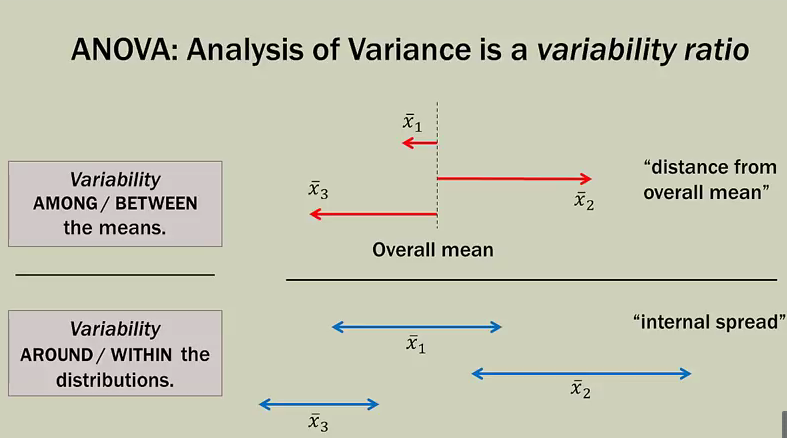
\includegraphics[width=0.8\linewidth,keepaspectratio]{anv7}
\end{center}
\end{frame}

%%%%%%%%%%%%%%%%%%%%%%%%%%%%%%%%%%%%%%%%%%%%%%%%%%%%%%%%%%%
\begin{frame}[fragile]\frametitle{Analysis of Variance (ANOVA)}
Total variance has two components.
\begin{center}
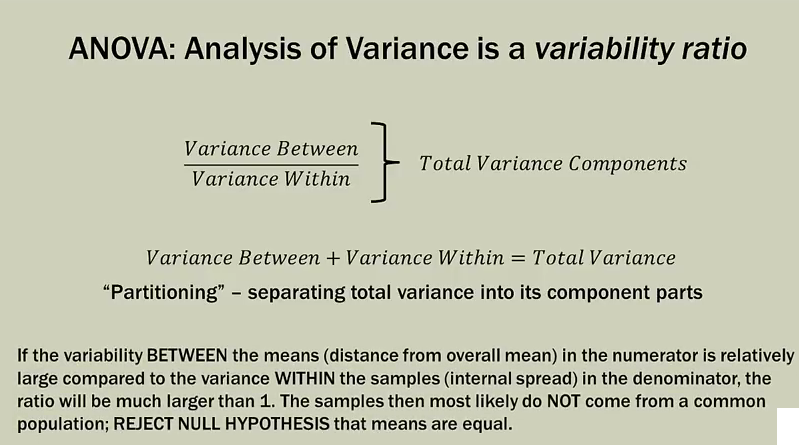
\includegraphics[width=0.8\linewidth,keepaspectratio]{anv8}
\end{center}
\end{frame}

%%%%%%%%%%%%%%%%%%%%%%%%%%%%%%%%%%%%%%%%%%%%%%%%%%%%%%%%%%%
\begin{frame}[fragile]\frametitle{Analysis of Variance (ANOVA)}
\begin{center}
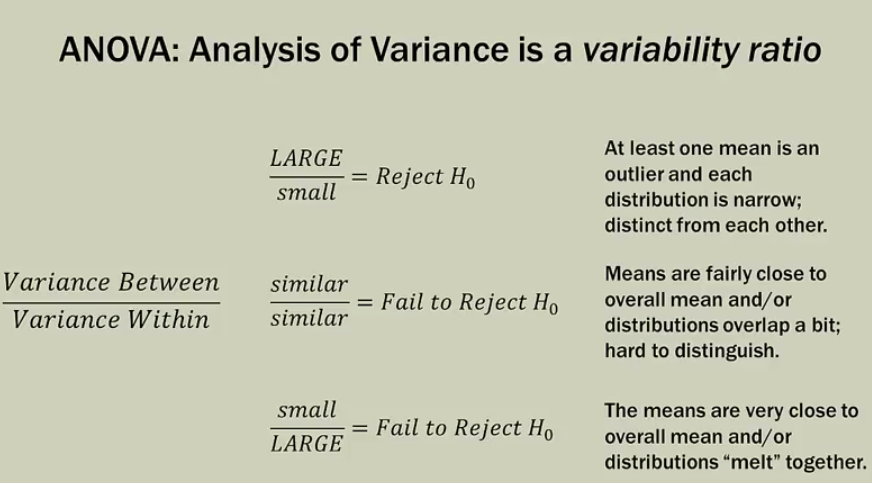
\includegraphics[width=0.8\linewidth,keepaspectratio]{anv9}
\end{center}
\end{frame}

%%%%%%%%%%%%%%%%%%%%%%%%%%%%%%%%%%%%%%%%%%%%%%%%%%%%%%%%%%
\begin{frame}[fragile]\frametitle{Analysis of Variance (ANOVA)}
\begin{center}
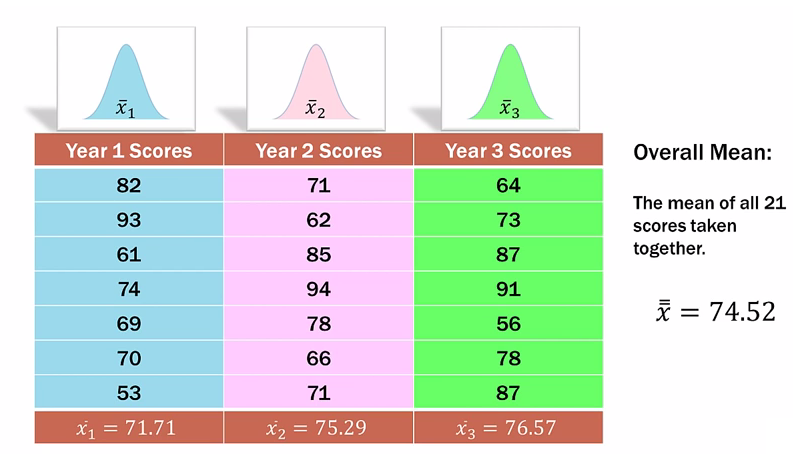
\includegraphics[width=0.8\linewidth,keepaspectratio]{anv11}
\end{center}
\end{frame}

%%%%%%%%%%%%%%%%%%%%%%%%%%%%%%%%%%%%%%%%%%%%%%%%%%%%%%%%%%%
\begin{frame}[fragile]\frametitle{Analysis of Variance (ANOVA)}
\begin{center}
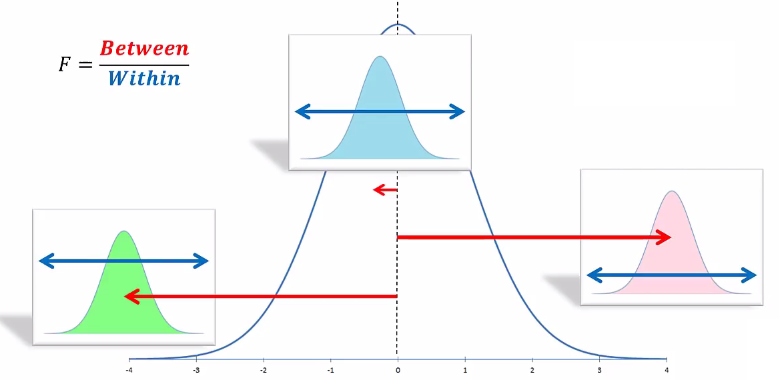
\includegraphics[width=0.8\linewidth,keepaspectratio]{anv10}
\end{center}
\end{frame}

%  https://www.youtube.com/watch?v=JgMFhKi6f6Y

%
%
%%%%%%%%%%%%%%%%%%%%%%%%%%%%%%%%%%%%%%%%%%%%%%%%%%%%%%%%%%%
%\begin{frame}[fragile]\frametitle{Analysis of Variance (ANOVA)}
%SS is variance without averaging
%\begin{center}
%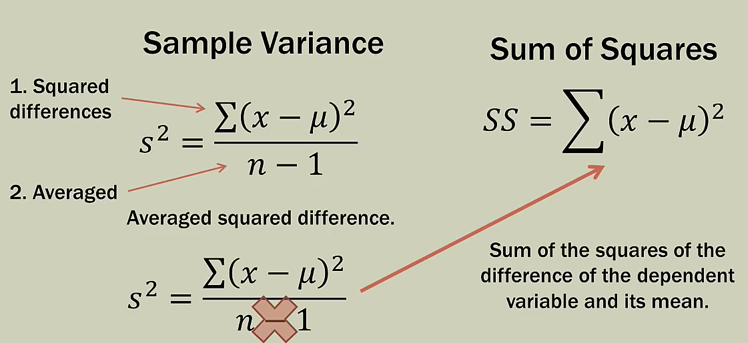
\includegraphics[width=0.8\linewidth,keepaspectratio]{anv12}
%\end{center}
%\end{frame}
%
%%%%%%%%%%%%%%%%%%%%%%%%%%%%%%%%%%%%%%%%%%%%%%%%%%%%%%%%%%%
%\begin{frame}[fragile]\frametitle{Analysis of Variance (ANOVA)}
%Total SS = SSC (variance between) + SSE (variance within)
%\begin{center}
%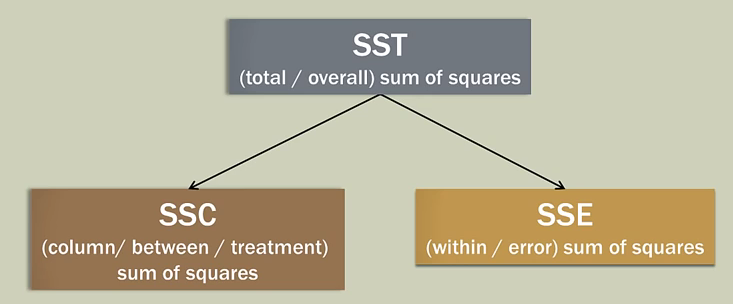
\includegraphics[width=0.8\linewidth,keepaspectratio]{anv13}
%\end{center}
%\end{frame}
%
%%%%%%%%%%%%%%%%%%%%%%%%%%%%%%%%%%%%%%%%%%%%%%%%%%%%%%%%%%%
%\begin{frame}[fragile]\frametitle{Analysis of Variance (ANOVA)}
%21 SS make up SST
%\begin{center}
%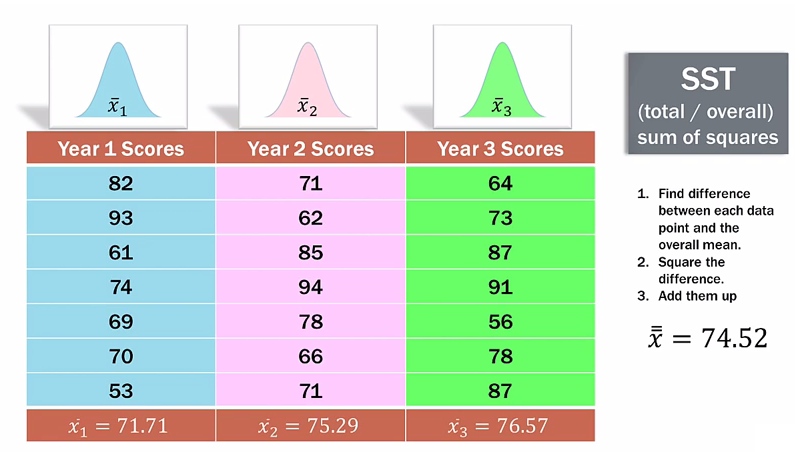
\includegraphics[width=0.8\linewidth,keepaspectratio]{anv14}
%\end{center}
%\end{frame}
%
%
%
%%%%%%%%%%%%%%%%%%%%%%%%%%%%%%%%%%%%%%%%%%%%%%%%%%%%%%%%%%%
%\begin{frame}[fragile]\frametitle{Analysis of Variance (ANOVA)}
%\begin{itemize}
%\item Analysis  of  variance  is  necessary  to  protect  researchers  from 
%excessive  risk  of  a  Type  I  error  in  situations  where  a  study  is 
%comparing more than two population means.   
%\item These situations would require a series of several t tests to evaluate 
%all of the mean differences.  (Remember, a t test can compare only 
%2 means at a time.)   
%\end{itemize}
%\end{frame}
%
%%%%%%%%%%%%%%%%%%%%%%%%%%%%%%%%%%%%%%%%%%%%%%%%%%%%%%%%%%%%
%\begin{frame}[fragile]\frametitle{Analysis of Variance (ANOVA)}
%\begin{itemize}
%\item ANOVA allows researcher to evaluate all of the mean differences 
%in  a  single  hypothesis  test  using  a  single  $\alpha$-level  and,  thereby, 
%keeps the risk of a Type I error under control no matter how many 
%different means are being compared. 
%\item Although  ANOVA  can  be  used  in  a  variety  of  different  research 
%situations,  this  chapter  presents  only  independent-measures 
%designs involving only one independent variable.  
%\end{itemize}
%\end{frame}
%
%%%%%%%%%%%%%%%%%%%%%%%%%%%%%%%%%%%%%%%%%%%%%%%%%%%%%%%%%%%
%\begin{frame}[fragile]\frametitle{Analysis of Variance (ANOVA)}
%\begin{center}
%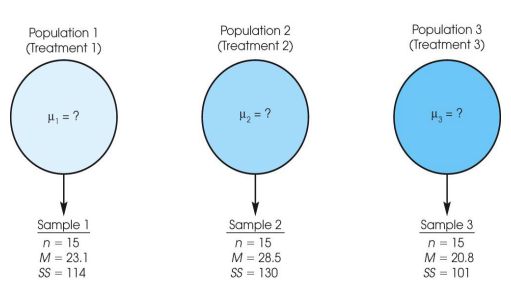
\includegraphics[width=\linewidth,keepaspectratio]{anova1}
%\end{center}
%\end{frame}
%
%
%%%%%%%%%%%%%%%%%%%%%%%%%%%%%%%%%%%%%%%%%%%%%%%%%%%%%%%%%%%
%\begin{frame}[fragile]\frametitle{Analysis of Variance (ANOVA)}
%\begin{itemize}
%\item The  null  hypothesis  for  ANOVA  states  that  for  the  general  population 
%there are no mean differences among the treatments being compared
%\item When  the  null  hypothesis  is  rejected,  the  conclusion  is  that  there  are 
%significant mean differences.  
%\end{itemize}
%\end{frame}
%
%%%%%%%%%%%%%%%%%%%%%%%%%%%%%%%%%%%%%%%%%%%%%%%%%%%%%%%%%%%
%\begin{frame}[fragile]\frametitle{Analysis of Variance (ANOVA)}
%\begin{itemize}
%\item However,  the  ANOVA  simply  establishes  that  differences  exist,  it  does 
%not indicate exactly which treatments are different.   
%\item For testing which treatments are significantly different from each other, 
%we can use multiple comparison tests. 
%\end{itemize}
%\end{frame}
%
%%%%%%%%%%%%%%%%%%%%%%%%%%%%%%%%%%%%%%%%%%%%%%%%%%%%%%%%%%%
%\begin{frame}[fragile]\frametitle{Analysis of Variance (ANOVA)}
%\begin{itemize}
%\item The test statistic for ANOVA is an F-ratio, which is a ratio of two sample 
%variances.    In  the  context  of  ANOVA,  the  sample  variances  are  called 
%mean squares, or MS values.   
%\item The  top  of  the  F-ratio  $MS_{between}$
%  measures  the  size  of  mean  differences 
%between  samples.    The  bottom  of  the  ratio  $MS_{within}$
%  measures  the 
%magnitude of differences that would be expected without any treatment 
%effects.  
%\end{itemize}
%\end{frame}
%
%%%%%%%%%%%%%%%%%%%%%%%%%%%%%%%%%%%%%%%%%%%%%%%%%%%%%%%%%%%
%\begin{frame}[fragile]\frametitle{Analysis of Variance (ANOVA)}
%Thus, the F-ratio has the same basic structure as the independent-
%measures t statistic. 
%\begin{center}
%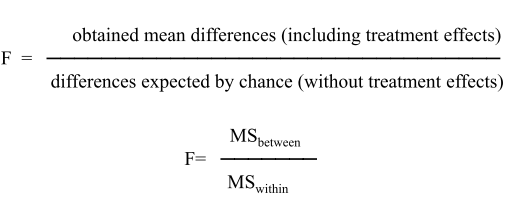
\includegraphics[width=0.5\linewidth,keepaspectratio]{anova2}
%\end{center}
%\end{frame}
%
%%%%%%%%%%%%%%%%%%%%%%%%%%%%%%%%%%%%%%%%%%%%%%%%%%%%%%%%%%%%
%\begin{frame}[fragile]\frametitle{Analysis of Variance (ANOVA)}
%\begin{itemize}
%\item A  large  value  for  the  F-ratio  indicates  that  the  obtained  sample 
%mean  differences  are  greater  than  would  be  expected  if  the 
%treatments had no effect. 
%\item Each  of  the  sample  variances,  MS  values,  in  the  F-ratio  is 
%computed using the basic formula for sample variance: $$ MS = \frac{SS}{df}$$
%\end{itemize}
%\end{frame}
%
%%%%%%%%%%%%%%%%%%%%%%%%%%%%%%%%%%%%%%%%%%%%%%%%%%%%%%%%%%%%
%\begin{frame}[fragile]\frametitle{Analysis of Variance (ANOVA)}
%To obtain the SS and df values, you must go through an analysis 
%that separates the total variability for the entire set of data into two 
%basic  components:  between-treatment  variability  (which  will 
%become  the  numerator  of  the  F-ratio),  and  within-treatment 
%variability (which will be the denominator).  
%
%\end{frame}
%
%%%%%%%%%%%%%%%%%%%%%%%%%%%%%%%%%%%%%%%%%%%%%%%%%%%%%%%%%%%%
%\begin{frame}[fragile]\frametitle{Analysis of Variance (ANOVA)}
%Considering these sources of variability, the structure of the F-ratio 
%becomes, 
%\begin{center}
%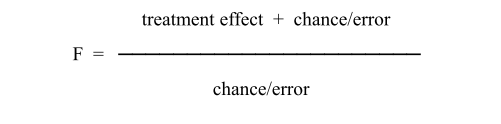
\includegraphics[width=0.5\linewidth,keepaspectratio]{anova3}
%\end{center}
%\end{frame}
%
%%%%%%%%%%%%%%%%%%%%%%%%%%%%%%%%%%%%%%%%%%%%%%%%%%%%%%%%%%
%\begin{frame}[fragile]\frametitle{Analysis of Variance (ANOVA)}
%\begin{itemize}
%\item When  the  null  hypothesis  is  true  and  there  are  no  differences 
%between treatments, the F-ratio is balanced.   
%\item That is, when the "treatment effect" is zero, the top and bottom of 
%the F-ratio are measuring the same variance.   
%\item In  this  case,  you  should  expect  an  F-ratio  near  1.00.    When  the 
%sample  data  produce  an  F-ratio  near  1.00,  we  will  conclude  that 
%there is no significant treatment effect. 
%\end{itemize}
%\end{frame}
%%%%%%%%%%%%%%%%%%%%%%%%%%%%%%%%%%%%%%%%%%%%%%%%%%%%%%%%%%%%
%\begin{frame}[fragile]\frametitle{Analysis of Variance (ANOVA)}
%\begin{itemize}
%\item On  the  other  hand,  a  large  treatment  effect  will  produce  a  large 
%value for the F-ratio.  Thus, when the sample data produce a large 
%\item F-ratio we will reject the null hypothesis and conclude that there 
%are significant differences between treatments. 
%\item To determine whether an F-ratio is large enough to be significant, 
%you must select an $\alpha$-level, find the df values for the numerator and 
%denominator of the F-ratio, and consult the F-distribution table to 
%find the critical value.  
%\end{itemize}
%\end{frame}


%%%%%%%%%%%%%%%%%%%%%%%%%%%%%%%%%%%%%%%%%%%%%%%%%%%%
%\begin{frame}[fragile]\frametitle{T-Test}
%The two normal probability distribution functions (p.d.f) stacked on top of each other look like this:
%\begin{center}
%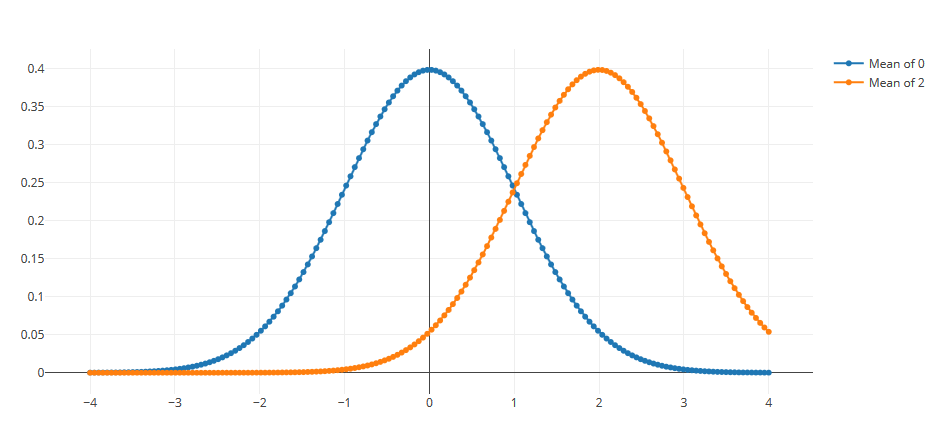
\includegraphics[width=\linewidth,keepaspectratio]{ttest1}
%\end{center}
%\end{frame}
%
%%%%%%%%%%%%%%%%%%%%%%%%%%%%%%%%%%%%%%%%%%%%%%%%%%%%
%\begin{frame}[fragile]\frametitle{T-Test}
%One sample T test: sample mean is equial to population mean $m = \mu$
%\begin{lstlisting}
%true_mu = 0
%
%onesample_results = scipy.stats.ttest_1samp(data1, true_mu)
%
%matrix_onesample = [
%    ['', 'Test Statistic', 'p-value'],
%    ['Sample Data', onesample_results[0], onesample_results[1]]
%]
%
%onesample_table = FF.create_table(matrix_onesample, index=True)
%py.iplot(onesample_table, filename='onesample-table')
%\end{lstlisting}
%\end{frame}
%
%


%
%\begin{frame}
%\frametitle{Two-sample comparisons}
%
%Suppose we are comparing samples from two populations, and we are
%interested in whether the two population means are equal.
%
%This is a very common setting.  Here are two specific examples:
%
%\begin{itemize}
%
%\item We are interested in comparing two treatments for high blood
%  pressure.  Each treatment lowers blood pressure on average by a
%  certain amount.  We would like to know the difference between the
%  two population ``treatment effects.''
%
%\item Visitors to a web site are shown one of two different
%  advertisements for the same product.  We are able to obtain the
%  fraction of the time that the user clicks on the ad (the ``click
%  rate'').  We would like to know the population value of the
%  difference in click rates.
%
%\end{itemize}
%
%\end{frame}
%
%\begin{frame}
%\frametitle{Two-sample comparisons}
%
%\begin{center}
%\scalebox{0.9}{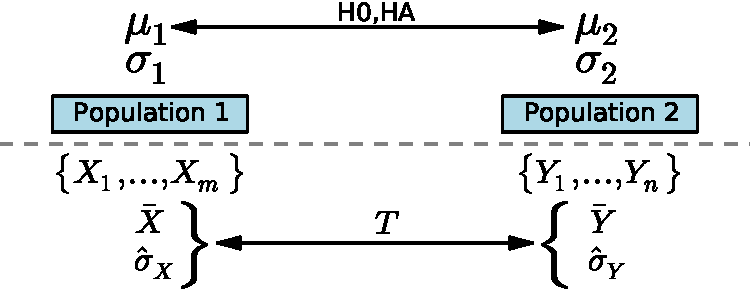
\includegraphics{015.pdf}}
%\end{center}
%
%\end{frame}
%
%\begin{frame}
%\frametitle{Two-sample comparisons}
%
%Let $X_1, \ldots, X_n$ denote the data from the first population, and
%$Y_1, \ldots, Y_m$ denote the data from the second population.  Let
%$\bar{X}$ and $\bar{Y}$ denote the two sample means.
%
%We can estimate the difference in population means using
%$\bar{X}-\bar{Y}$.  If the population means are $\mu_X$ and $\mu_Y$,
%then $\bar{X}-\bar{Y}$ is an unbiased estimate of the mean difference
%$\mu_X-\mu_Y$, i.e.
%
%$$ E(\bar{X}-\bar{Y}) = \mu_X - \mu_Y.
%$$
%
%\end{frame}
%
%
%\begin{frame}
%\frametitle{Two-sample comparisons}
%
%For testing, we can consider the \textcolor{purple}{null hypothesis}
%$\mu_X = \mu_Y$.
%
%As a test statistic, we can start with $D = \bar{X} - \bar{Y}$, but we
%will need to standardize it.
%
%Under the null hypothesis, $ED = 0$.  The variance of $D$ is 
%
%\begin{eqnarray*}
%{\rm var}(\bar{X} - \bar{Y}) &=& {\rm var}(\bar{X}) + {\rm
%  var}(-\bar{Y})\\ &=& {\rm var}(\bar{X}) + {\rm
%  var}(\bar{Y})\\ &=& \sigma_X^2/n + \sigma_Y^2/m.
%\end{eqnarray*}
%
%Thus the {\bf two-sample Z-statistic}
%
%$$
%T \equiv \frac{\bar{X} - \bar{Y}}{\sqrt{\sigma_X^2/n + \sigma_Y^2/m}}
%$$
%
%has a standardized distribution under the null
%hypothesis.
%
%\end{frame}
%
%
%\begin{frame}
%\frametitle{Two-sample comparisons}
%
%A test statistic value of $T=0$ is perfectly consistent with the null
%hypothesis.  Larger values of $|T|$ indicate increasing levels of
%evidence against the null hypothesis.
%
%The \textcolor{purple}{p-value} is the null distribution probability
%that as much evidence or more evidence against the null is observed
%(hypothetically, if the null hypothesis were true) than was actually
%observed:
%
%$$
%p = P_0(|T| \ge |T_{\rm obs}|)
%$$
%
%This is the {\bf 2-sided p-value} -- there are similar expressions for
%one-sided (right and left tail) p-values.
%
%\end{frame}
%
%
%\begin{frame}
%\frametitle{Two-sample comparisons}
%
%Treating the test statistic $T$ as having a standard normal
%distribution under the null hypothesis, the p-value can be computed as
%
%\begin{eqnarray*}
%P_0(|T| \ge |T_{\rm obs}|) &=& P_0(T \ge |T_{\rm obs}|) + P_0(T \le
%-|T_{\rm obs}|)\\ &=& 2\cdot P(T \le -|T_{\rm obs}|),
%\end{eqnarray*}
%
%where $P_0(T \ge |T_{\rm obs}|) = P_0(T \le -|T_{\rm obs}|)$ due to the
%symmetry of the normal distribution.
%
%\end{frame}
%
%
%\begin{frame}
%\frametitle{Acceptance/rejection of hypotheses}
%
%An alternative framework (to p-values) for hypothesis testing is based
%on the idea that a null hypothesis is \textcolor{purple}{rejected} if
%$|T|$ is sufficiently large, and otherwise is
%\textcolor{purple}{accepted}.  
%
%In this setting, there are two ways we can make the correct decision
%and two ways we can make the wrong decision:
%
%\bigskip
%
%\begin{center}
%\begin{tabular}{lll}
%              & Accept $H_0$ & Reject $H_0$\\\hline
%$H_0$ is true & Correct      & Type I error\\
%$H_A$ is true & Type II error & Correct\\\hline
%\end{tabular}
%\end{center}
%
%\bigskip
%
%The \textcolor{purple}{level} of a hypothesis test is the probability
%that a type I error occurs.
%
%\end{frame}
%
%\begin{frame}
%\frametitle{Acceptance/rejection of hypotheses}
%
%Suppose the sampling distribution of $T$ under the null hypothesis is
%standard normal and we reject the null hypothesis when $|T|>2$.
%
%There are two ways we can reject -- either when $T>2$ or when $T<-2$.
%Each of these events has probability 0.025, so the type I error is
%0.05.
%
%\bigskip
%
%\begin{center}
%\scalebox{0.6}{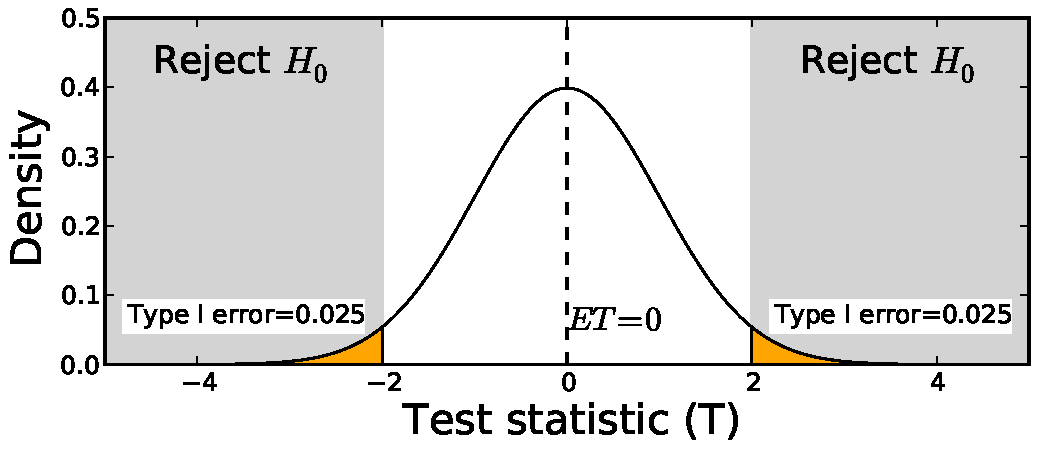
\includegraphics{049.pdf}}
%\end{center}
%
%
%\end{frame}
%
%
%\begin{frame}
%\frametitle{Two-sample tests with unknown variances}
%
%If the variances in the $X$ and $Y$ populations are unknown, we can
%use the estimated variance
%
%$$
%\hat{\sigma}_X^2/n + \hat{\sigma}_Y^2/m.
%$$
%
%In this case the test statistic is approximately t-distributed with
%the following degrees of freedom:
%
%$$ \frac{(\sigma_X^2/n + \sigma_Y^2/m)^2}{(\sigma_X^2/n)^2/(n-1) +
%(\sigma_Y^2/m)^2/(m-1)}.
%$$
%
%\end{frame}
%
%
%\begin{frame}
%\frametitle{Power of hypothesis tests}
%
%\begin{center}
%The \textcolor{purple}{power} of a hypothesis test is the probability
%of rejecting the null hypothesis when the alternative hypothesis is
%true.
%
%\end{center}
%
%Here are two equivalent ways of describing the power:
%
%\begin{itemize}
%
%\item The power is the probability of getting a p-value below a
%  defined value (usually 0.05) when the alternative hypothesis is
%  true.
%
%\item If the test statistic $T$ is standardized under the null
%  hypothesis, the power is the probability that $T$ exceeds the
%  critical value (usually $2$) when the alternative hypothesis is true.
%
%\end{itemize}
%
%The power depends on the sample size and the \textcolor{purple}{effect
%  size}, which is a measure of how distinguishable the null and
%alternative hypotheses are from each other.
%
%\end{frame}
%
%\begin{frame}
%\frametitle{Power of two-sample hypothesis tests}
%
%The effect size is related to two other quantities:
%
%\begin{itemize}
%
%\item The \textcolor{purple}{raw (unstandardized) effect size} is the
%  difference in population means of the two groups being compared.
%
%\item The \textcolor{purple}{response variability} is a summary of the
%  differences among individuals that are not related to their
%  treatment status.
%
%\end{itemize}
%
%Power is positively related to the raw effect size and is inversely
%related to response variability.
%
%\textcolor{blue}{\bf Example:} We have more power to detect a given
%treatment effect if everyone's blood pressure drops by 5 units, than
%if half of the subjects have a 10 unit decline and half of the
%subjects have no decline at all (even though the average decline is 5
%units in both cases).
%
%\end{frame}
%
%\begin{frame}
%\frametitle{Power of two-sample hypothesis tests}
%
%The two-sample Z-test statistic can be rewritten as
%
%$$
%T = \sqrt{m+n}\frac{\bar{X} - \bar{Y}}{\sqrt{\sigma_X^2/q_X + \sigma_Y^2/q_Y}},
%$$
%
%where $q_X = n/(n+m)$ and $q_Y = m/(n+m)$ are the proportions of the
%overall sample drawn from each of the two populations.
%
%Most test statistics can be written in this form
%
%$$ \sqrt{\rm total\;sample\;size}\times{\rm a\;``stable\;value''}
%$$
%
%Here the total sample size is $m+n$ and the ``stable
%value'' is
%
%$$
%\frac{\bar{X} - \bar{Y}}{\sqrt{\sigma_X^2/q_X + \sigma_Y^2/q_Y}}.
%$$
%
%\end{frame}
%
%\begin{frame}
%\frametitle{Power of two-sample hypothesis tests}
%
%By the central limit theorem, we know that under the null hypothesis,
%as $m$ and $n$ grow, $T$ becomes increasingly well approximated by a
%standard normal distribution.
%
%Under the alternative hypothesis, we have
%
%$$ E\frac{\bar{X} - \bar{Y}}{\sqrt{\sigma_X^2/q_X + \sigma_Y^2/q_Y}} =
%\frac{\mu_X - \mu_Y}{\sqrt{\sigma_X^2/q_X + \sigma_Y^2/q_Y}} \equiv
%\Delta.
%$$
%
%Thus the expected test statistic is approximately equal to
%$\sqrt{m+n}\cdot\Delta$ -- it continues to grow (at ``rate''
%$\sqrt{m+n}$) as the sample size grows.
%
%\end{frame}
%
%
%\begin{frame}
%\frametitle{Power of two-sample hypothesis tests}
%
%Here we see the density function of the test statistic, in a case
%where its expected value is $ET=2.5$:
%
%\begin{center}
%\scalebox{0.6}{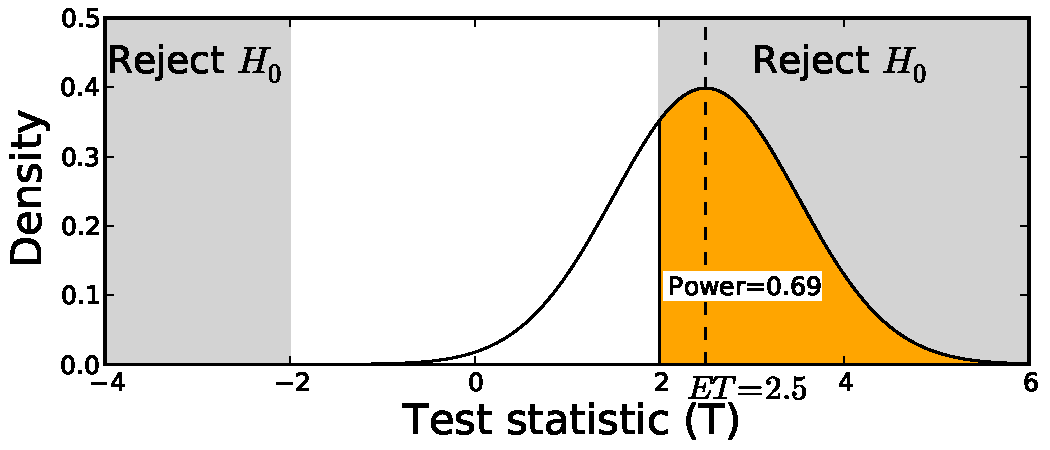
\includegraphics{047.pdf}}
%\end{center}
%
%If the test statistic falls in the grey region, we reject the null
%hypothesis.  The power is the probability of this happening, indicated
%by the orange region.
%
%Note that the standard deviation of the test statistics is one.
%
%\end{frame}
%
%
%\begin{frame}
%\frametitle{Power of two-sample hypothesis tests}
%
%For the two-sample problem, we can use $\delta = \mu_X - \mu_Y$ as the
%raw (unstandardized) effect size.
%
%The power is
%
%$$
%P(|T| \ge 2) = P(T \ge 2) + P(T \le -2).
%$$
%
%The first summand is
%
%\begin{eqnarray*}
%P(T\ge 2) &=& P\left(\sqrt{m+n}\frac{\bar{X} -
%  \bar{Y}}{\sqrt{\sigma_X^2/q_X + \sigma_Y^2/q_Y}} \ge 2\right)\\ &=&
%P\left(\sqrt{m+n}\frac{\bar{X} - \bar{Y} -
%  \delta}{\sqrt{\sigma_X^2/q_X + \sigma_Y^2/q_Y}}
%\ge\right.\\&&\;\;\;\;\;\; \left. 2 -
%\delta\sqrt{(m+n)/(\sigma_X^2/q_X + \sigma_Y^2/q_Y)}\right).
%\end{eqnarray*}
%
%\end{frame}
%
%
%\begin{frame}
%\frametitle{Power of two-sample hypothesis tests}
%
%Under the alternative hypothesis, $\bar{X} - \bar{Y} - \delta$ has
%mean zero, so 
%
%$$ \sqrt{m+n}\frac{\bar{X} - \bar{Y} - \delta}{\sqrt{\sigma_X^2/q_X +
%\sigma_Y^2/q_Y}}
%$$
%
%can be treated as being standard normal.  Thus
%
%$$ P(T> 2) = 1 - P\left(Z \le 2 - \delta\sqrt{(m+n)/(\sigma_X^2/q_X +
%\sigma_Y^2/q_Y)}\right),
%$$
%
%which can be obtained from a standard normal probability table.
%
%A similar calculation can be used to get an expression for $P(T \le
%-2)$.
%
%Note that as $\delta$ grows and/or $m+n$ grows and/or $\sigma_X$ and
%$\sigma_Y$ shrink, the power gets closer and closer to 1.
%
%\end{frame}
%
%
%\begin{frame}
%\frametitle{Power (determining sample size)}
%
%We often need to assess what sample size would be required to detect
%an effect in a particular situation.
%
%For example, we may be interested in detecting a treatment effect in
%which a drug lowers a particular quantity by two units on average.  We
%may be also be willing to assume (for the purposes of power analysis)
%that this quantity varies with a standard deviation of 3 units (for
%both treated and untreated subjects). Suppose also
%that we intend to carry out our study using equal numbers of treated
%and untreated subjects.
%
%In the notation of the preceding slides, we have
%
%\begin{itemize}
%
%\item $\mu_X-\mu_Y = 2$ (This is the raw, or unstandardized treatment
%  effect, where X is the untreated group and Y is the treated group.)
%
%\item $\sigma_X = \sigma_Y = 3$ (This is the variability of
%  individual subjects' blood pressures around the mean of the group
%  they belong to (either treated or untreated.)
%
%\item $q_X = q_Y = 1/2$ (This is our ``design decision'' to use
%  equal numbers of treated and untreated subjects.)
%
%\end{itemize}
%
%\end{frame}
%
%
%\begin{frame}
%\frametitle{Power (determining sample size)}
%
%So the ``stable value'' $\Delta$ is
%
%$$
%\Delta = \frac{2}{\sqrt{9/(1/2) + 9/(1/2)}} = 1/3
%$$
%
%Thus the test-statistic will have mean value equal to
%
%\begin{center}
%$\sqrt{m+n}\cdot\Delta = \sqrt{2n}/3$
%\end{center}
%
%To reject the null hypothesis at the usual (two-sided $\alpha=0.05$)
%level, we need the test statistic to be greater than 2.  Thus we have
%$\sqrt{2n}/3>2$, or $n>18$ to get 50\% power.
%
%If we want 80\% power, then we need to solve
%
%\vspace{-0.5cm}
%
%$$
%0.8 = P(T>2) = P(T-ET>2-ET) = P(Z>2-\sqrt{2n}/3).
%$$
%
%Since the 20${\rm th}$ percentile of a standard normal distribution is
%$-0.84$, this gives us $2-\sqrt{2n}/3 = -0.84$, so we
%need $n=36$ to get 80\% power.
%
%\end{frame}
%
%
%\begin{frame}
%\frametitle{Power (determining effect size)}
%
%A different type of power analysis comes up when the sample size is
%fixed, and we are asked to determine what effects can be detected at
%that sample size.
%
%Suppose we are given that a comparison of two treatments will involve
%20 treated subjects, and 40 untreated subjects, and we are willing to
%assume (for the purposes of power analysis), that the standard
%deviation within the treated subjects is 1 and the standard deviation
%within the untreated subjects is 2.
%
%We have
%
%\begin{itemize}
%
%\item $\sigma_X = 1$, $\sigma_Y = 2$
%
%\item $q_X = 1/3$, $q_Y = 2/3$
%
%\item $\sqrt{m+n} = \sqrt{60} \approx 7.75$.
%
%\end{itemize}
%
%We now need to determine what values of $\delta = \mu_x-\mu_y$ would
%allow us to reject the null hypothesis with reasonably high frequency.
%
%\end{frame}
%
%
%\begin{frame}
%\frametitle{Power (determining effect size)}
%
%The expected value of the test statistic is
%
%$$ \sqrt{m+n}\cdot\Delta \approx
%7.75\cdot\frac{\mu_x-\mu_y}{\sqrt{1/(1/3) + 2/(2/3)}} \approx
%2.6\delta.
%$$
%
%To get 80\% power, we need
%
%$$
%0.8 = P(T>2) = P(T-ET>2-ET) = P(Z>2-2.6\delta).
%$$
%
%Thus we have $2-2.6\delta = -0.84$, so $\delta = 1.09$ is
%required.
%
%\end{frame}
%
